%%%%%%%%%%%%%%%%%%%%%%%%%%%%%%%%%%%%%%%%%%%%%%%%%%%%%%%%%%%%%%%%%%%%%%%%%%%%%%%%%%%%%%%%%%%%%%%%%%%%%%%%%%%%%%%%%%%%%%%%%%%%%%%%%%%%%%%%%%%%%%%%%%%%%%%%%%%%%%%%%%%%%%%%%%%%%%%%%%%%
\chapter{Characterisation and estimation of the Standard Model backgrounds}
\label{sec:BackgroundEstimation}
After the application of the candidate track selection explained in the previous section the background arising from Standard Model processes is dramatically reduced.
Only two events in the simulated \WJets sample remain.
One of these originates from an unreconstructed muon, and one from an unreconstructed electron.
That means, it can still happen sometimes that an electron, muon or tau fails reconstruction.
Due to the limited size of the simulated \WJets dataset (15 times smaller than the number of events expected from \WJets processes during 2012 data taking), 
it is not possible to rely on a full simulation-based estimation of the leptonic background.
The underlying mechanism of the non-reconstruction of a lepton and the corresponding methods to estimate the leptonic background will be in detail explained in Section~\ref{sec:LeptonicBkg}.

Furthermore, there is the possibility that a track is reconstructed out of a set of hits that do not origin from only one single particle.
Such tracks are called ``fake tracks''. 
Background tracks arising from the wrong combination of hits will be explained in the following section~\ref{sec:FakeBkg}.
%The composition of the background after the candidate track selection is shown in Fig.~\ref{fig:BkgComposition}.
%\begin{figure}[!bt]
%  \centering 
%  \begin{tabular}{c}
%    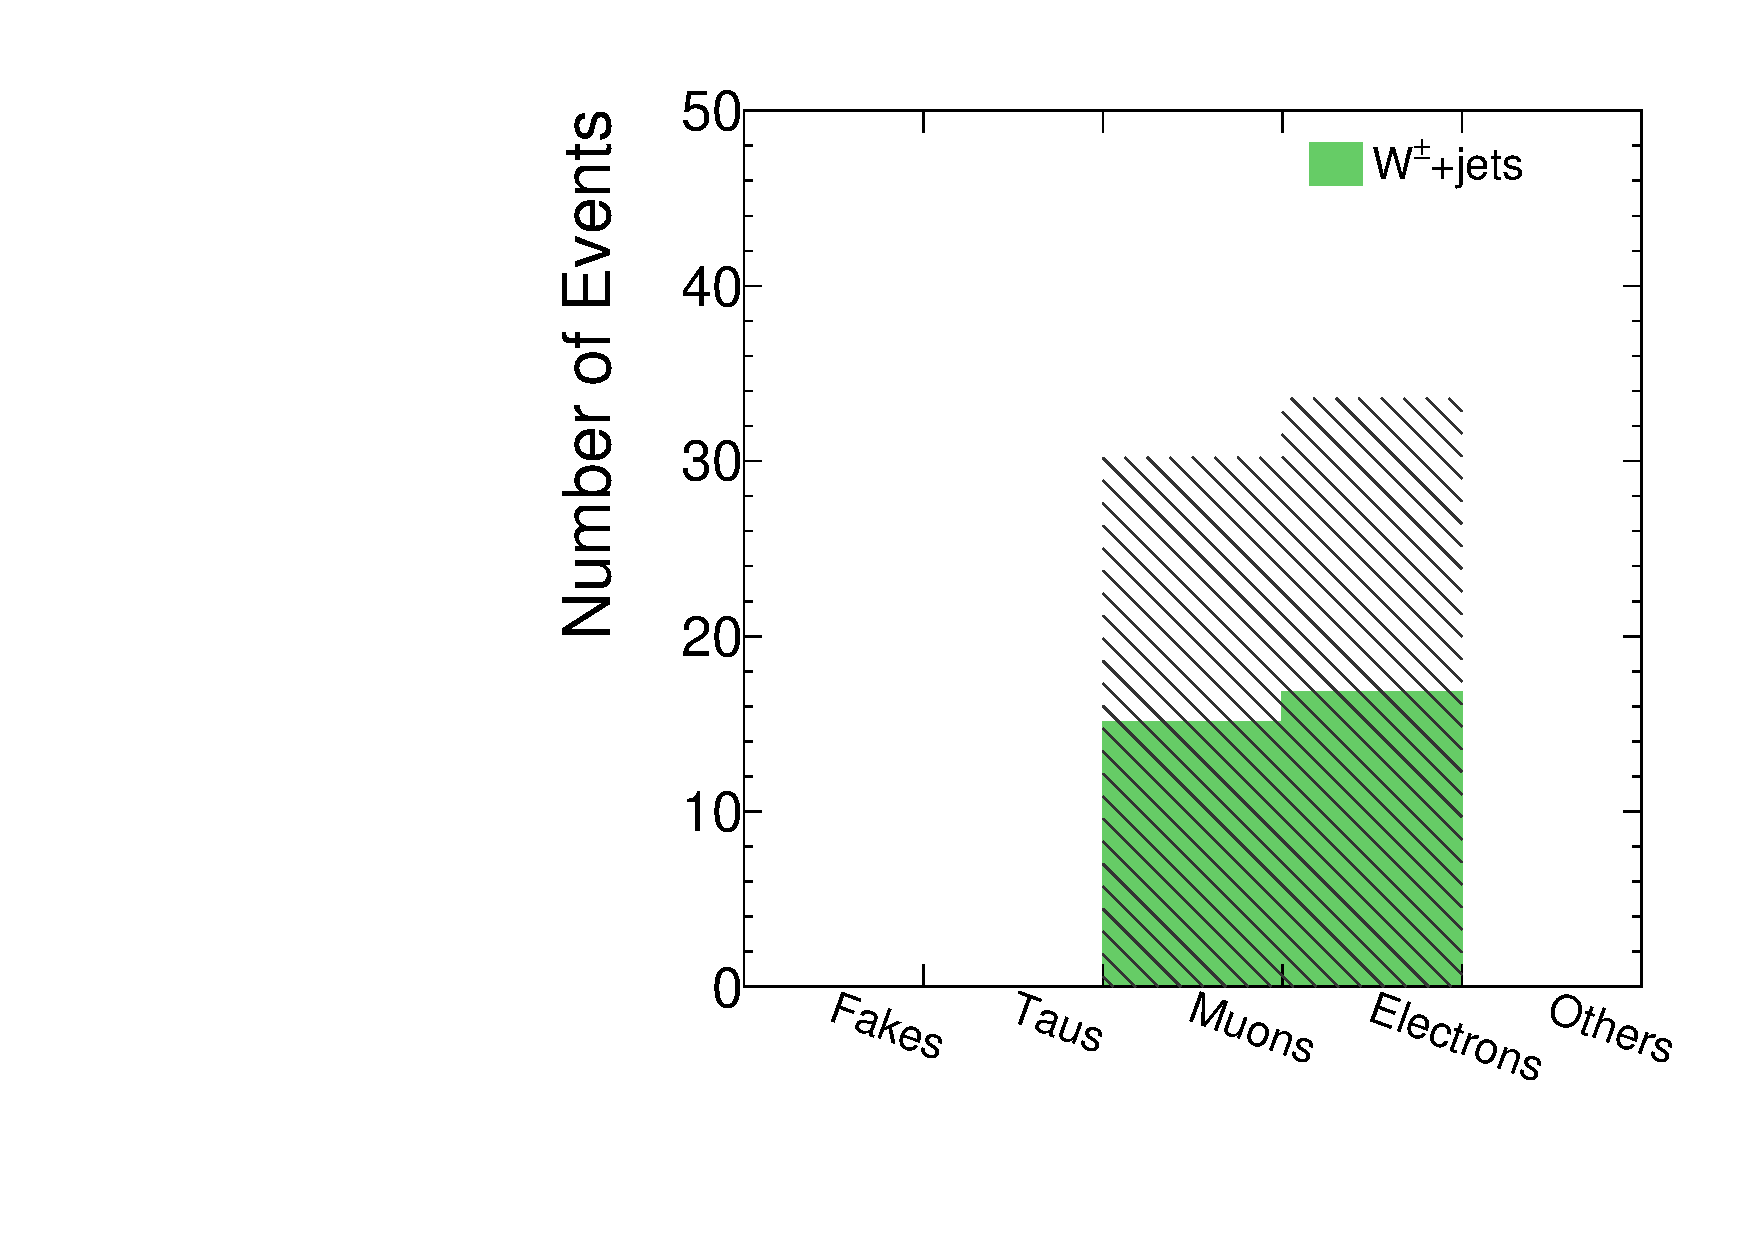
\includegraphics[width=0.49\textwidth]{figures/analysis/AnalysisSelection/chiTracksfullSelectionTrigger_Wjets/htrackgenParticleSmallRange_lin.pdf}
%    %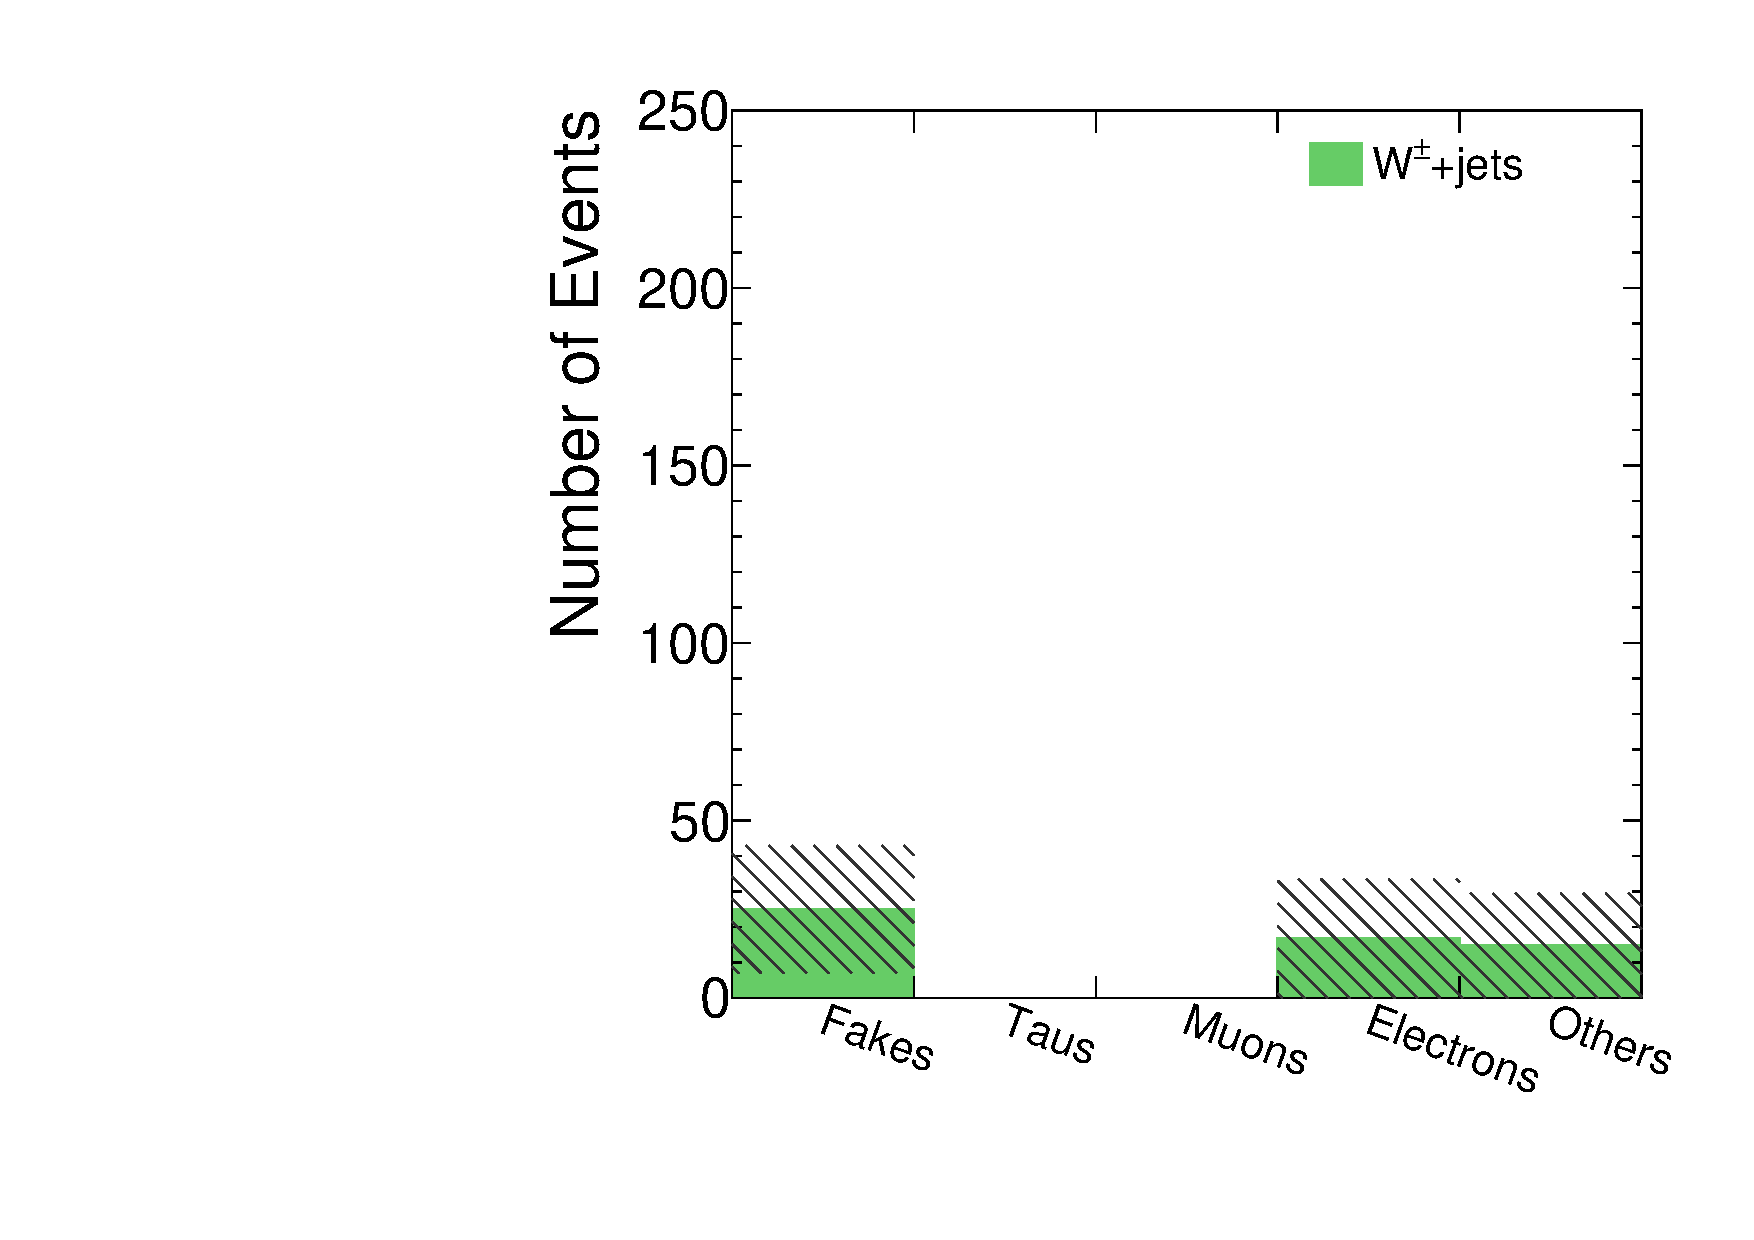
\includegraphics[width=0.49\textwidth]{figures/analysis/AnalysisSelection/chiTracksfullSelectionPlusIasTrigger_Wjets/htrackgenParticleSmallRange_lin.pdf}
%  \end{tabular}
%  \caption{Background composition in the simulated \WJets dataset after the full candidate track selection.
%           The statistical uncertainty is depicted by the hashed grey area.
%           Given the limited size of the simulated \WJets dataset, the uncertainty of the composition is accordingly large.}
%  \label{fig:BkgComposition}
%\end{figure}
%This composition can change significantly when imposing further selection cuts on \pt and \ias.
%The definition of the signal region will be, however, addressed within the optimisation of the search sensitivity in Section~\ref{sec:Optimisation}.
%To get a feeling how the composition of the background is affected by further cuts on one of the main variables, 
%the background composition is also shown with the candidate track selection plus an additional \ias cut of 0.05.
%It can be seen that the fake background is less reduced by an additional selection cut on \ias.
It needs to be mentioned that the fake background is contributing through all SM processes, not only via \WJets processes.
Still, the characteristics of fake tracks can be studied using only \WJets.
The limited quality of the $dE/dx$ simulation enforces anyways a data-based background estimation method.



%%%%%%%%%%%%%%%%%%%%%%%%%%%%%%%%%%%%%%%%%%%%%%%%%%%%%%%%%%%%%%%%%%%%%%%%%%%%%%%%%%%%%%%%%%%%%%%%%%%%%%%%%%%%%%%%%%%%%%%%%%%%%%%%%%%%%%%%%%%%%%%%%%%%%%%%%%%%%%%%%%%%%%%%%%%%%%%%%%%%
%%%%%%%%%%%%%%%%%%%%%%%%%%%%%%%%%%%%%%%%%%%%%%%%%%%%%%%%%%%%%%%%%%%%%%%%%%%%%%%%%%%%%%%%%%%%%%%%%%%%%%%%%%%%%%%%%%%%%%%%%%%%%%%%%%%%%%%%%%%%%%%%%%%%%%%%%%%%%%%%%%%%%%%%%%%%%%%%%%%%
\section{Fake background}
\label{sec:FakeBkg}
Fake tracks are tracks which are not reconstructed out of the trajectory of one single particle.
The rate with which this wrong reconstruction occurs is of course highly restrained by the quality cuts on $\chi^2$ and the vertex compatibility of the track reconstruction algorithm.
Details on the reconstruction algorithm at CMS can be found in Section~\ref{FIXME}.
The probability of reconstructing a fake track is strongly correlated with the number of hits in the tracker system.
This can be seen in Fig~\ref{fig:NValidFakes}, where the distribution of the number of hits of fakes is depicted.
\begin{figure}[!t]
  \centering 
  \begin{tabular}{c}
    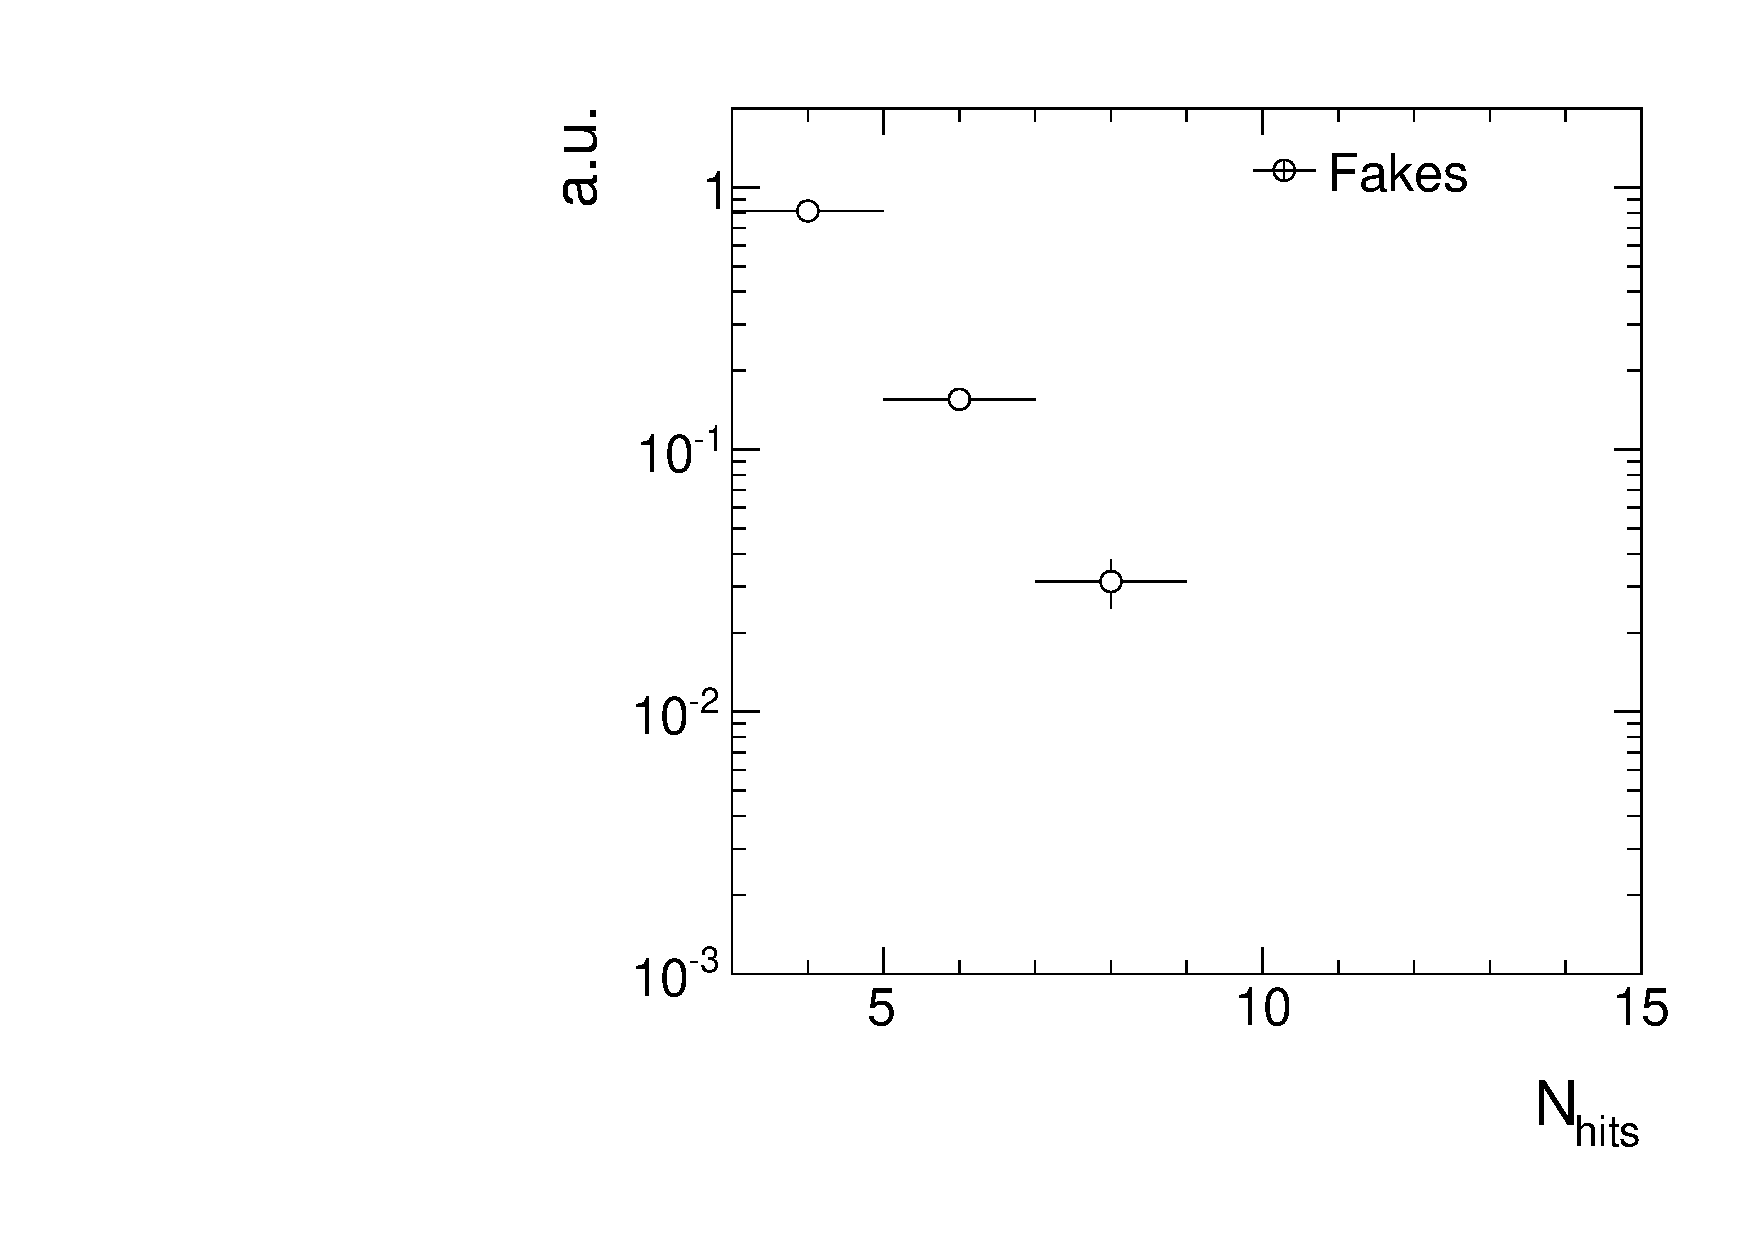
\includegraphics[width=0.49\textwidth]{figures/analysis/Background/NValidForFakes_chiTracksfullSelectionNoTriggerCuts.pdf}
  \end{tabular}
  \caption{Normalised distribution of the number of hits for fake tracks after the candidate track selection from Section~\ref{sec:CandidateTrackSelection}.}
  \label{fig:NValidFakes}
\end{figure}
There are almost no fakes with a number of hits larger than six.
In simulation, fake tracks are defined as tracks which cannot be matched to a generator-level particle within a distance of $\Delta R < 0.01$.

Fakes are efficiently suppressed by the requirements of no missing middle or inner hits and the compatibility with the primary vertex.
Unfortunately, wrongly reconstructed tracks which pass these criteria, do also easily pass the $\ecalo<5\gev$ requirement with high efficiency.\\

In this analysis, the estimation of the fake background is split into two parts.
First, the background is estimated inclusively in \ias.
Second, to be able to optimise later in the variable \ias, the \ias distribution is taken from a fake enriched control region.

\subsection*{Inclusive fake background estimation}
The inclusive background estimation follows closely the background estimation method done in~\cite{bib:CMS:DT_Thesis,bib:CMS:DT_8TeV_AN}.
It aims to determine the probability of having a fake track in an event that pass the full track selection (besides the \ias criterium).
This probability will be called the fake rate.

The inclusive fake background is estimated with the help of $Z\rightarrow\mu\bar{\mu}$ and $Z\rightarrow e\bar{e}$ events from data.
Selecting clean \Zlep events can be done with high efficiency by requiring two well reconstructed muons or electrons, that are opposite in charge and for which the invariant mass is around the $Z$-boson mass of $\sim90\gev$.
Putting on top the candidate track selection described in Section~\ref{sec:CandidateTrackSelection}, the selected track must be a fake.

The selection of two well reconstructed muons and electrons is done with the single-muon and single-electron datasets listed in Table~\ref{tab:ElectronMuonCRDatasets}.
\renewcommand{\arraystretch}{1.5}
\begin{table}[!h]
\centering
\caption{Datasets used for the determination of the fake rate.}
\label{tab:ElectronMuonCRDatasets}
\makebox[0.99\textwidth]{
\begin{tabular}{lr}
\multicolumn{2}{c}{} \\
\toprule
Dataset  & Luminosity [\fbinv]   \\
\midrule
/SingleMu/Run2012A-22Jan2013-v1/AOD        &  0.876 \\
/SingleMu/Run2012B-22Jan2013-v1/AOD        &  4.405 \\
/SingleMu/Run2012C-22Jan2013-v1/AOD        &  7.040 \\
/SingleMu/Run2012D-22Jan2013-v1/AOD        &  7.369 \\ 
\midrule
/SingleElectron/Run2012A-22Jan2013-v1/AOD  &  0.876 \\
/SingleElectron/Run2012B-22Jan2013-v1/AOD  &  4.412 \\
/SingleElectron/Run2012C-22Jan2013-v1/AOD  &  7.050 \\
/SingleElectron/Run2012D-22Jan2013-v1/AOD  &  7.368 \\
\bottomrule
\end{tabular}}
\end{table}  
For the $Z\rightarrow\mu\bar{\mu}$ selection an event is required to have two muons with $\pt>25\gev$ and $|\eta|<2.4$.
To supress background from cosmic muons, the distance from the primary vertex must be less than $|d0|<0.2\cm$ in radial and $|dz|<0.5\cm$ in longitudinal direction.
To supress background arising from jets that fake muons, various quality criteria are apllied. 
Thus, it is required that there is at least one hit in the muon detector and at least two hits in different detector planes.   
Concerning the track of the muon in the tracker system, at minimum one hit in the pixel tracker and at least six hits in the full tracker system is required. 
An isolation criterium is applied that requires the sum of transverse momenta in a cone of $\Delta R<0.4$ of all PF particles to be less than 12\%.
Finally, the muons are required to be opposite in charge and that their invariant mass is between $80-100\gev$.
The $Z\rightarrow\mu\bar{\mu}\,+\,\text{fake track}$ selection is summarised in Table~\ref{tab:FakeMuonSample}.
\renewcommand{\arraystretch}{1.4}
\begin{table}[!h]
\centering
\caption{Event selection cuts for the muons\,+\,fake control sample to estimate the inclusive fake background.}
\label{tab:FakeMuonSample}
\makebox[0.99\textwidth]{
\begin{tabular}{l|l l }
\multicolumn{3}{c}{} \\
\toprule
\multirow{12}{*}{\makecell[l]{Event based \\ selection}}       &  Two global muons with & $\pt>25\gev$ \\
                                                               &                        & $|\eta|<2.4$ \\
                                                               &                        & $\sum\limits_{\Delta R<0.4} \pt^{\text{PF particle}}/\pt(\mu)<0.12$ \\
                                                               &                        & $\left.\frac{\chi^2}{ndof}\right\rvert_{\text{global track}}<10$ \\
                                                               &                        & $|d0|<0.2\cm$  \\
                                                               &                        & $|dz|<0.5\cm$  \\
                                                               &                        & $\geq$ 1 hit in the muon detector  \\
                                                               &                        & $\geq$ 2 hits in different muon detector planes  \\
                                                               &                        & $\geq$ 1 hit in the pixel detector  \\
                                                               &                        & $\geq$ 6 hits in the tracker system  \\
                                                               &  \multicolumn{2}{l}{Muons opposite in charge}                                     \\
                                                               &  \multicolumn{2}{l}{$80\gev<M_{\text{inv}}\left(\mu_1,\mu_2  \right)<100\gev$}        \\

\midrule

\multirow{4}{*}{\makecell[l]{Candidate track\\ selection}}    &  Good quality selection \\
                                                              &  Kinematic selection    \\
                                                              &  Lepton/jet veto        \\   
                                                              &  Isolation selection    \\  
\bottomrule
\end{tabular}}
\end{table}

In order to select $Z\rightarrow e\bar{e}$ events in data, the two electrons are required to have \mbox{$\pt>25\gev$}, $|\eta|<2.5$ and no missing hits in the inner layers of the tracker.
Furthermore, the electrons need to pass a conversion veto to reduce background arising from photon conversions (as described in~\cite{bib:CMS:ConversionVeto_PAS}).
An isolation requirement is applied similar to the muon isolation criterium with a reduced cut of 15\%.
The electron identification is further based on a multivariate technique developed within~\cite{bib:CMS:ElectronMVA} that exploits electron characteristics about the track quality, the ECAL cluster shapes, and the combination about the measurements in the tracker and in the ECAL.
Again, also the two electrons must be opposite in charge and their invariant mass must be between $80-100\gev$.
A summary of the $Z\rightarrow e\bar{e}\,+\,\text{fake track}$ event selection can be found in Table~\ref{tab:FakeElectronSample}.\\
\renewcommand{\arraystretch}{1.4}
\begin{table}[!h]
\centering
\caption{Event selection cuts for the electrons\,+\,fake control sample to estimate the inclusive fake background.}
\label{tab:FakeElectronSample}
\makebox[0.99\textwidth]{
\begin{tabular}{l|l l }
\multicolumn{3}{c}{} \\
\toprule
\multirow{8}{*}{\makecell[l]{Event based \\ selection}}        &  Two Electrons with    & $\pt>25\gev$ \\
                                                               &                        & $|\eta|<2.5$ \\
                                                               &                        & $\sum\limits_{\Delta R<0.4} \pt^{\text{PF particle}}/\pt(e)<0.15$ \\
                                                               &                        & pass conversion veto    \\
                                                               &                        & no missing tracker hits  \\
                                                               &                        & good MVA electron as defined in \cite{bib:CMS:ElectronMVA}  \\
                                                               &  \multicolumn{2}{l}{Electrons opposite in charge}                                     \\
                                                               &  \multicolumn{2}{l}{$80\gev<M_{\text{inv}}\left(e_1,e_2  \right)<100\gev$}        \\

\midrule

\multirow{4}{*}{\makecell[l]{Candidate track\\ selection}}    &  Good quality selection \\
                                                              &  Kinematic selection    \\
                                                              &  Lepton/jet veto        \\   
                                                              &  Isolation selection    \\  
\bottomrule
\end{tabular}}
\end{table}  

When applying a \Zlep selection plus the candidate track selection, the selected track should be a fake.
If this is indeed the case can be tested on simulated \Zlep events.
As can be seen in Fig.~\ref{fig:BkgComposition}, a reasonable purity in fake tracks can be achieved by applying the candidate track selection on top of the \Zlep selection.
\begin{figure}[!b]
  \centering 
  \begin{tabular}{c}
    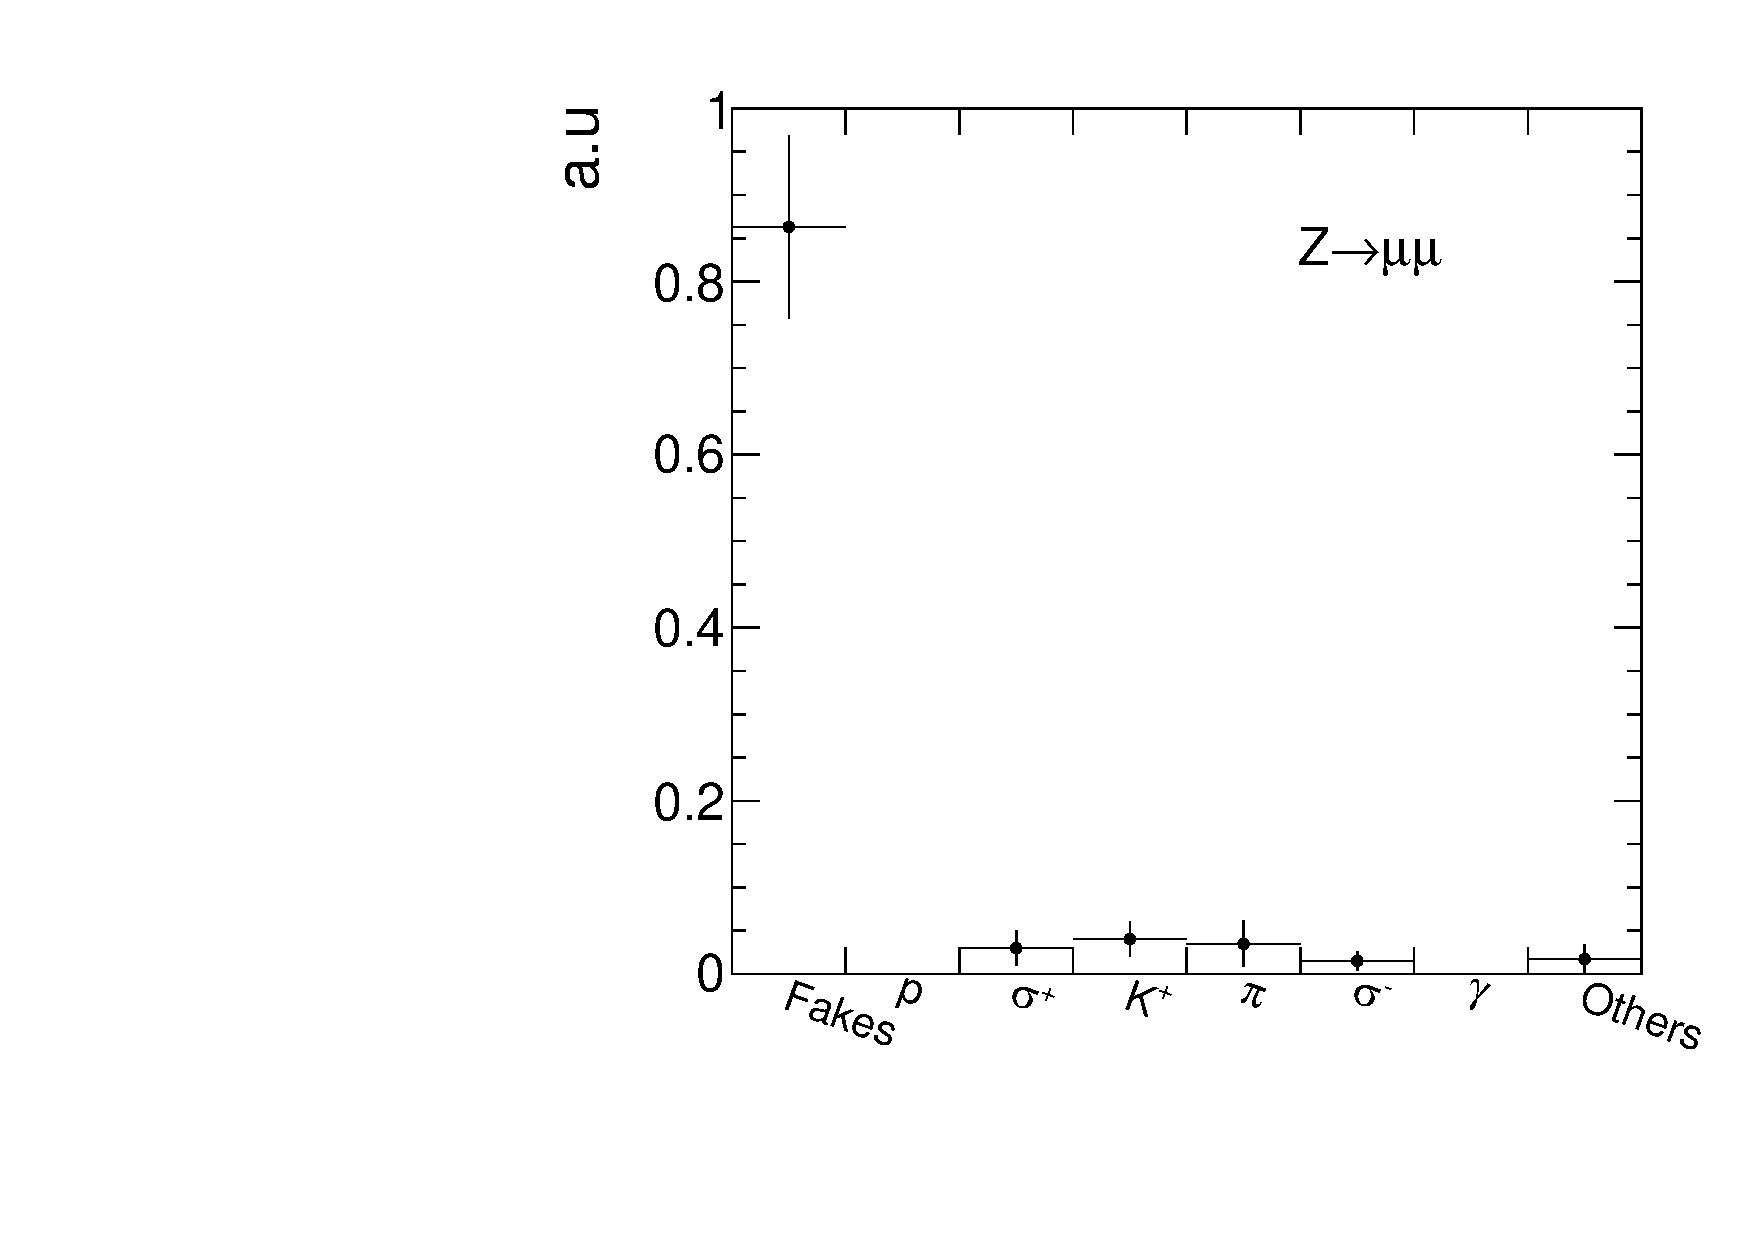
\includegraphics[width=0.49\textwidth]{figures/analysis/Background/ParticleCompositionInFakeCS_Mu.pdf}
    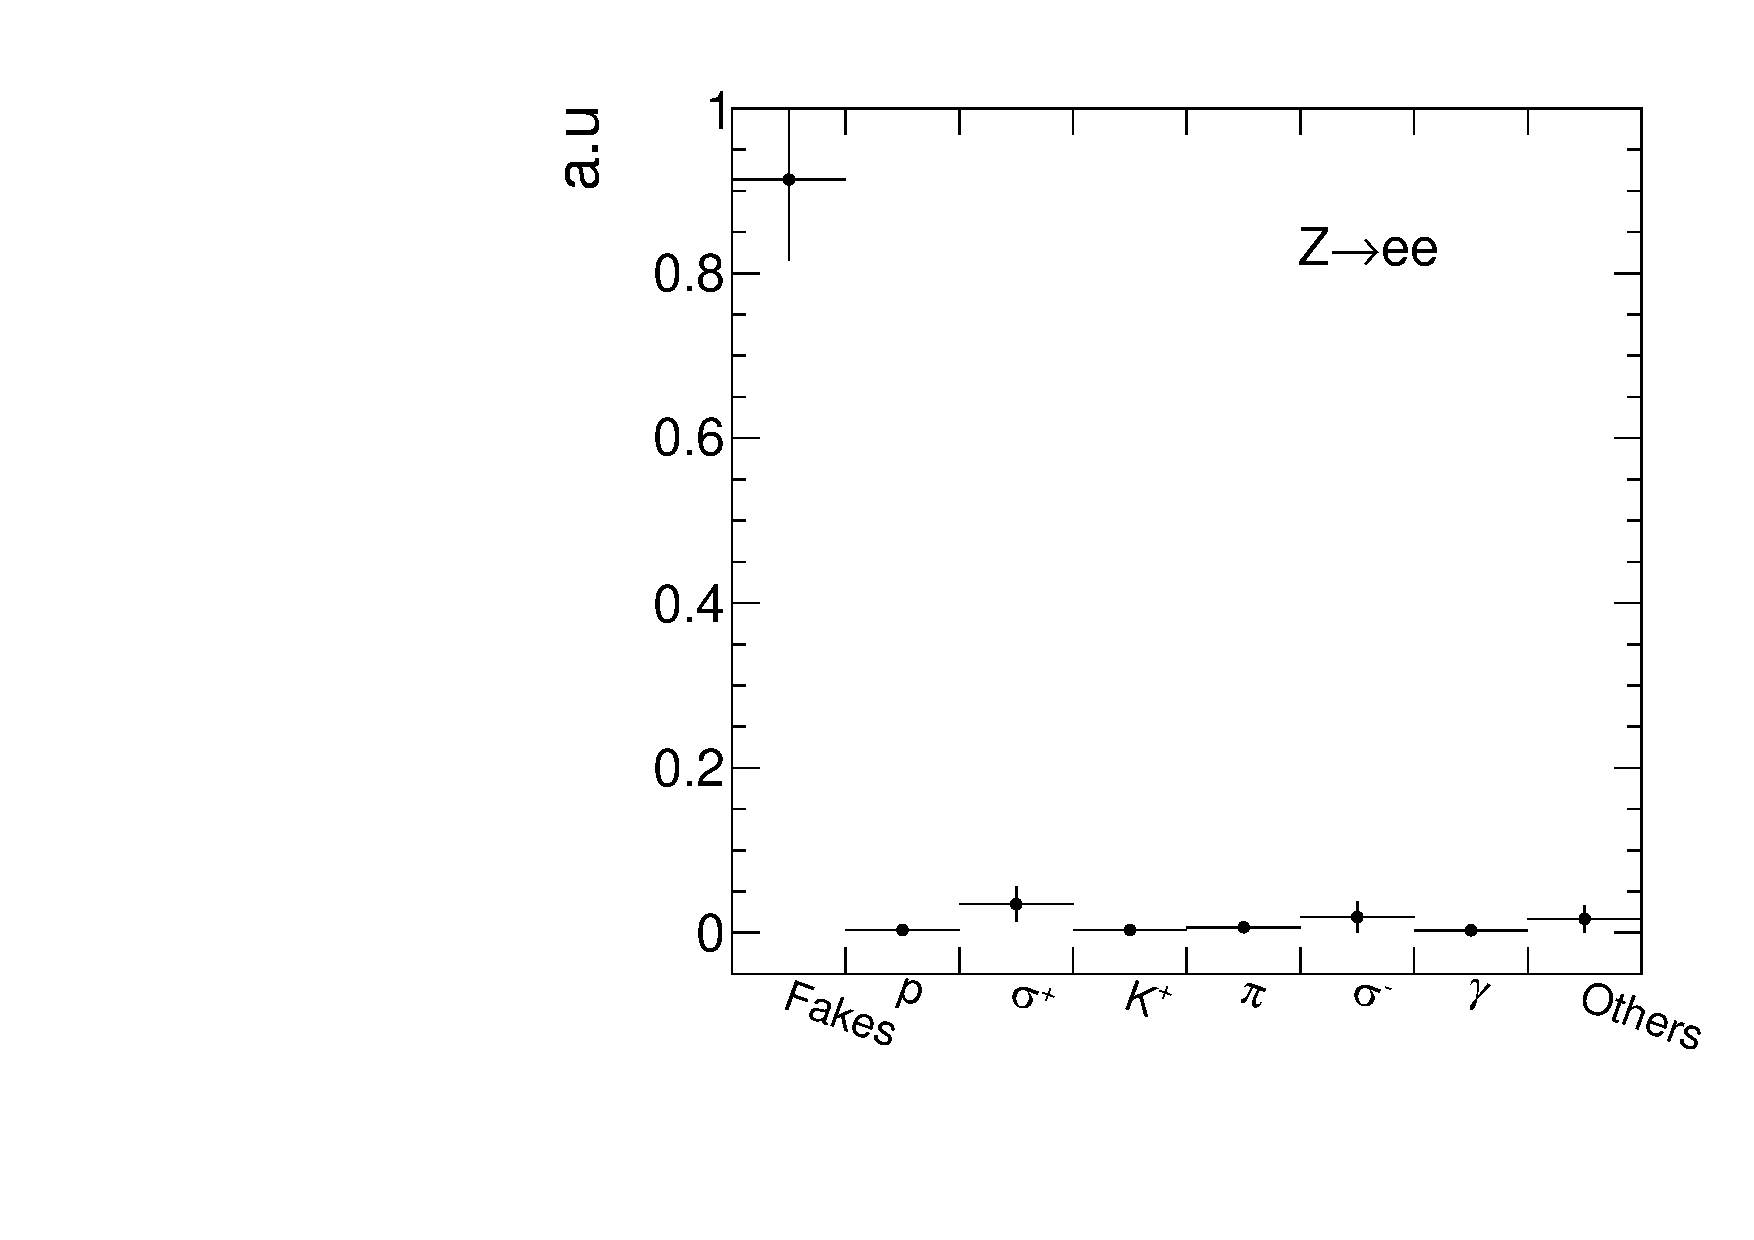
\includegraphics[width=0.49\textwidth]{figures/analysis/Background/ParticleCompositionInFakeCS_Ele.pdf}
  \end{tabular}
  \caption{Generator-level particle matched to the selected track with the selection described in Table~\ref{tab:FakeMuonSample} (left) and Table~\ref{tab:FakeElectronSample} (right). ``Fake'' mean that no corresponding generator-level particle could be found. }
  \label{fig:BkgComposition}
\end{figure}
In simulated $Z\rightarrow\mu\bar{\mu}$ events, a purity of 88\%, whereas in simulated $Z\rightarrow e\bar{e}$ events a purity of 92\% of fake tracks can be achieved.


As already mentioned, the fake rate is defined as the probability that an event contains a fake track that fulfils the candidate track selection criteria listed in Section~\ref{sec:CandidateTrackSelection}.
Thus, for the \Zlep datasets it is defined as the number of events passing the full selection described in Table~\ref{tab:FakeMuonSample} (Table~\ref{tab:FakeElectronSample}) divided by the number of events that pass only the event based selection in Table~\ref{tab:FakeMuonSample} (Table~\ref{tab:FakeElectronSample})
\begin{equation*}
\rho_{\text{fake}} = \frac{N_{Z\rightarrow ll}^{\text{cand trk selection}}}{N_{Z\rightarrow ll}}
\end{equation*}
The fake rate for the candidate track selection is e.g. $\left( 6.86 \pm 0.25 \right) \cdot 10^{-5}$. 
This is of course not the final result as the optimisation in \pt will add an additional \pt selection cut to the candidate track selection.

Within~\cite{bib:CMS:DT_Thesis,bib:CMS:DT_8TeV_AN}, it was checked that the fake rate is constant for different processes.
This is shown in Fig.~\ref{fig:FakeRate} where the fake rate is depicted for the most important SM processes.
\begin{figure}[!b]
  \centering 
  \begin{tabular}{c}
    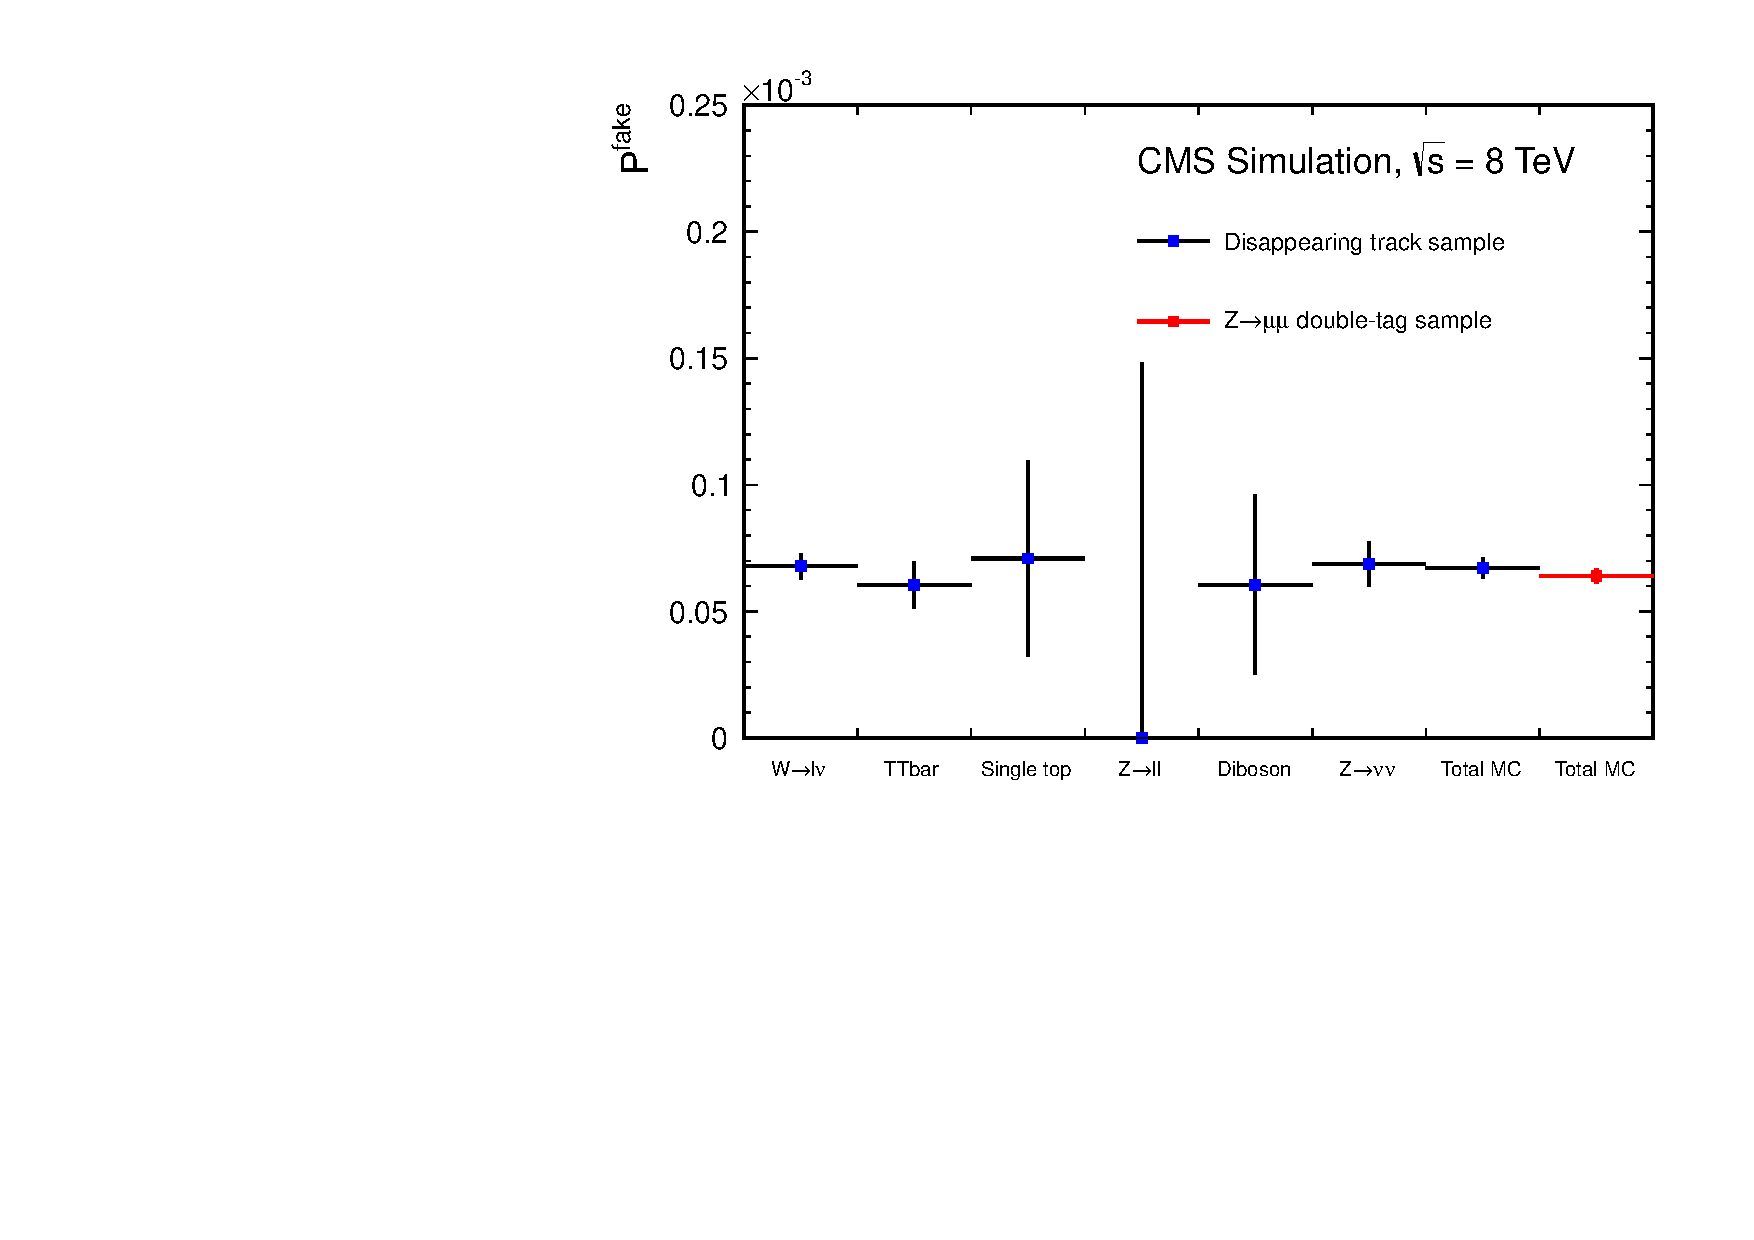
\includegraphics[width=0.79\textwidth]{figures/analysis/Background/fakeTrkRates.pdf}
  \end{tabular}
  \caption{Fake track rate estimated in \cite{bib:CMS:DT_Thesis,bib:CMS:DT_8TeV_AN} for tracks with four hits. Taken from \cite{bib:CMS:DT_8TeV_AN} }
  \label{fig:FakeRate}
\end{figure}
Since the fake rate is constant for different SM processes, the fake rate determined on the \Zlep dataset can be generalised for all SM background possibily contributing to this search.
Thus, the inclusive fake background can be estimated by multiplying the fake rate with the number of events selected in the MET dataset after the event based selection from Section~\ref{sec:EventBasedSelection}
\begin{equation*}
N^{\text{fake, inclusive in I$_{\text{as}}$}}_{\text{bkg}} = \rho_{\text{fake}} \cdot N_{\text{event based selection}}^{\text{MET}}.
\end{equation*}
Given the number of events after the event based selection of $N_{\text{event based selection}}^{\text{MET}} = 1.38\cdot10^6$ and the fake rate cited above, 
the inclusive fake background can be estimated to $94.7\pm3.4$ for the candidate track selection.

It should again be mentioned that the inclusive fake background estimation will be only inclusive in \ias not in \pt.
That means that after the definition of the signal region, $N^{\text{fake, inclusive in I$_{\text{as}}$}}_{\text{bkg}}$ is determined with the additional optimal \pt selection.
Possible differences between the fake rate in \Zlep events and other SM processes will be estimated with simulated events and taken as systematic uncertainty into account (see Section~\ref{sec:FakeRateUncertainty}).

To receive information about the selection efficiency of an \ias selection criterium, information about the \ias shape of fake tracks is needed.
How to receive this information will be explained in the next section.
%%%%%%%%%%%%%%%%%%%%%%%%%%%%%%%%%%%%%%%%%%%%%%%%%%%%%%%%%%%%%%%%%%%%%%%%%%%%%%%%%%%%%%%%%%%%%%%%%%%%%%%%%%%%%%%%%%%%%%%%%%%%%%%%%%%%%%%%%%%%%%%%%%%%%%%%%%%%%%%%%%%%%%%%%%%%%%%%%%%%
\subsection*{\ias shape of fake background}
Information of the energy release per path length for fake tracks should not be taken from simulated samples as the simulation of $dE/dx$ is not reliable (see Fig.~\ref{fig:Data-MC-Dedx_MIPs}).
To get still knowledge about the \ias shape of fake tracks, a control region CR$_{\ias}^{\text{fake}}$ is defined that is enriched with fakes and shows the same \ias distribution as fake tracks in the signal region.

To enrich fake tracks, it is possible to invert the selection cuts of the number of missing middle and inner hits, i.e. requiring at least one missing inner or middle hit $\left( N_{\text{miss}}^{\text{inner}} +N_{\text{miss}}^{\text{middle}}>0\right)$ .
This can be seen in Fig~\ref{fig:NMissInnerAndMiddle}, where the distribution of the number of missing inner plus missing middle hits is shown for fakes compared to the leptonic background for simulated \WJets events.
\begin{figure}[!b]
  \centering 
  \begin{tabular}{c}
    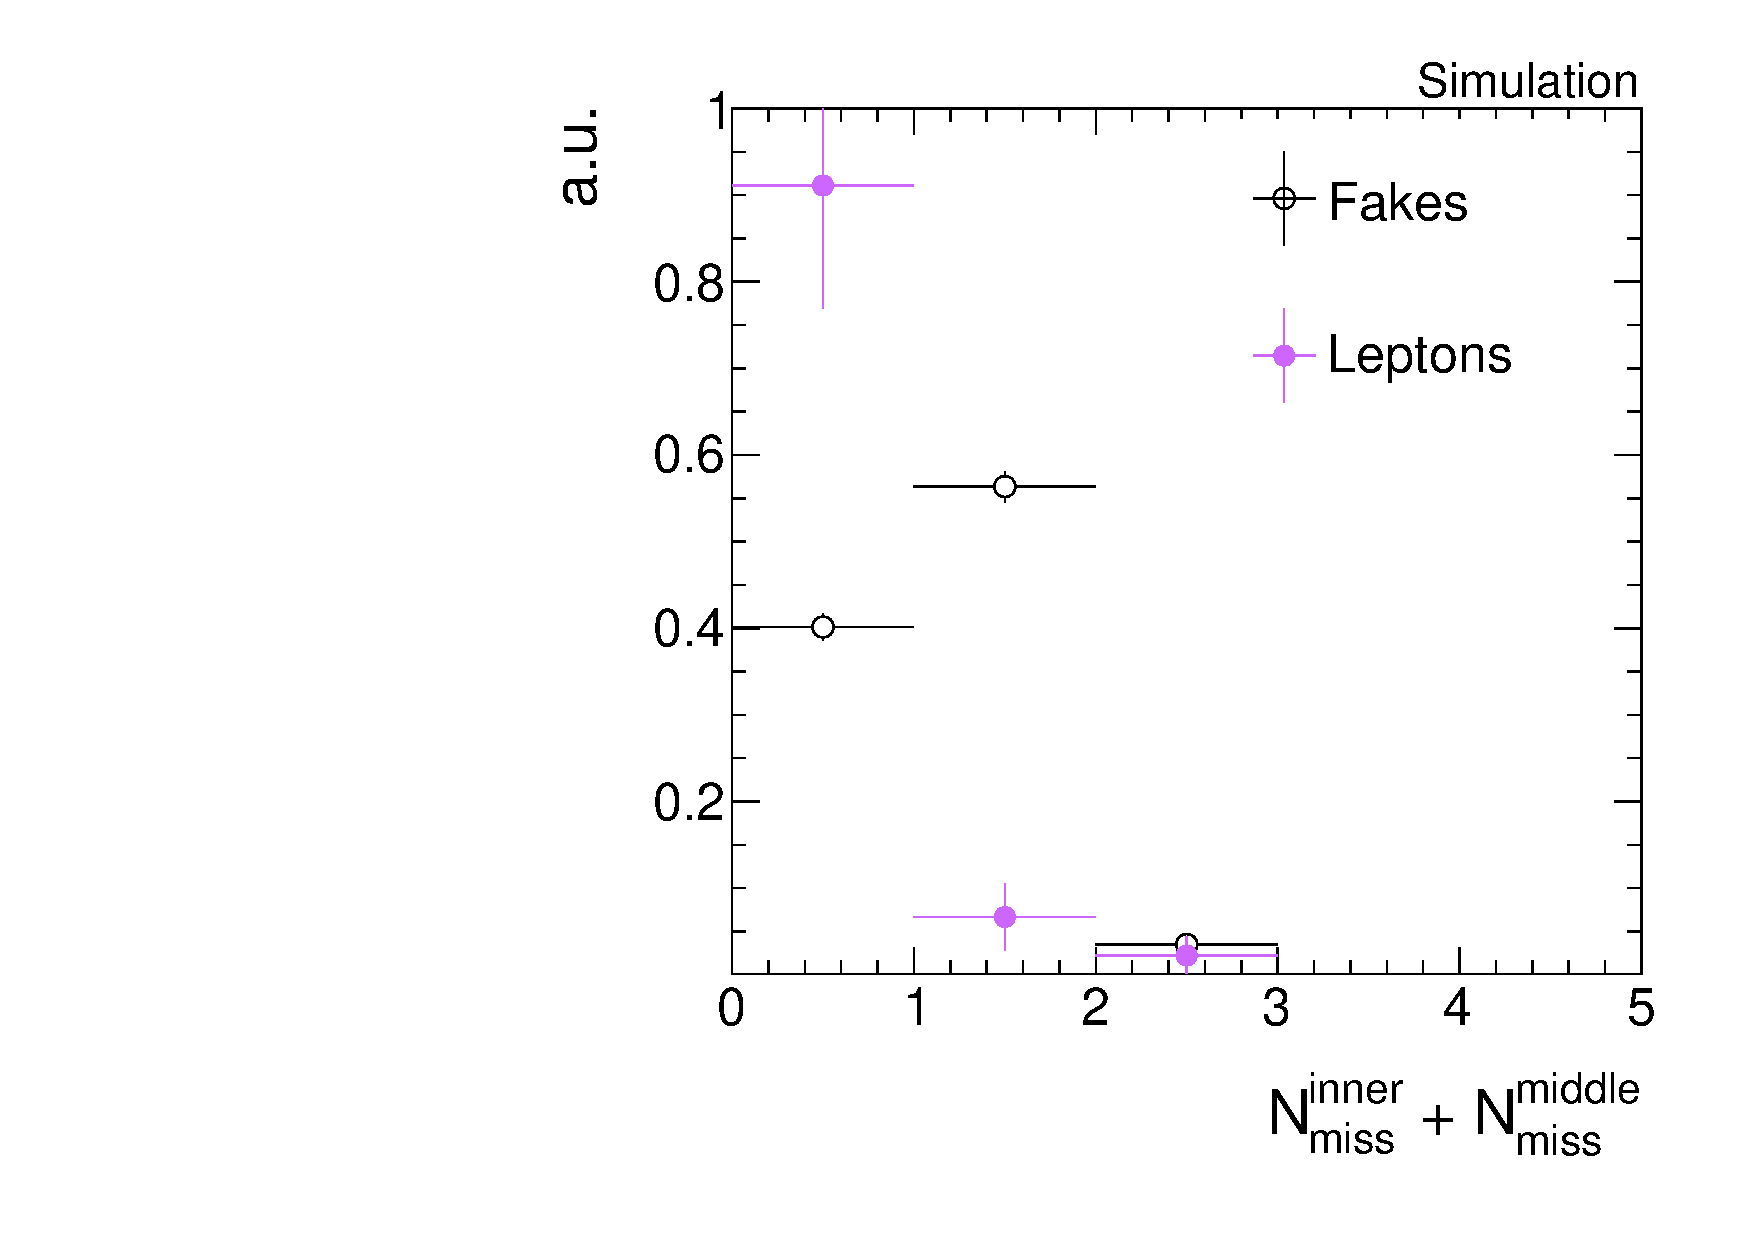
\includegraphics[width=0.49\textwidth]{figures/analysis/Background/NLostInnerPlusMiddleForAllBkg_chiTracksQCDsupressionTrigger.pdf}
  \end{tabular}
  \caption{Normalised number of missing inner plus missing middle hits for fake and leptonic tracks for the full candidate track selection with the selection requirements on $N_{\text{miss}}^{\text{inner}}$ and $N_{\text{miss}}^{\text{middle}}$ removed. The trigger requirements and QCD supression cuts were removed to enhance the statistical precisison.}
  \label{fig:NMissInnerAndMiddle}
\end{figure}

Of course, it needs also to be checked wether the \ias shape in CR$_{\ias}^{\text{fake}}$ is comparable to the \ias shape in the signal region.
As the exact definition of the signal region will be addressed during optimisation, this test is be done for various \pt selection cuts.

The comparison of the \ias shape of fake tracks can of course only be done on simulation.
Thus, simulated \WJets events are used to select fake tracks in both region.
A compariosn of the shape for the candidate track selection and the CR$_{\ias}^{\text{fake}}$ is shown in Fig~\ref{fig:IasSRCRFakes}.
It can be seen that indeed an excellent purity of around 99\% of fakes can be achieved in the \ias fake control region CR$_{\ias}^{\text{fake}}$.


\begin{figure}[!t]
  \centering 
  \begin{tabular}{c}
    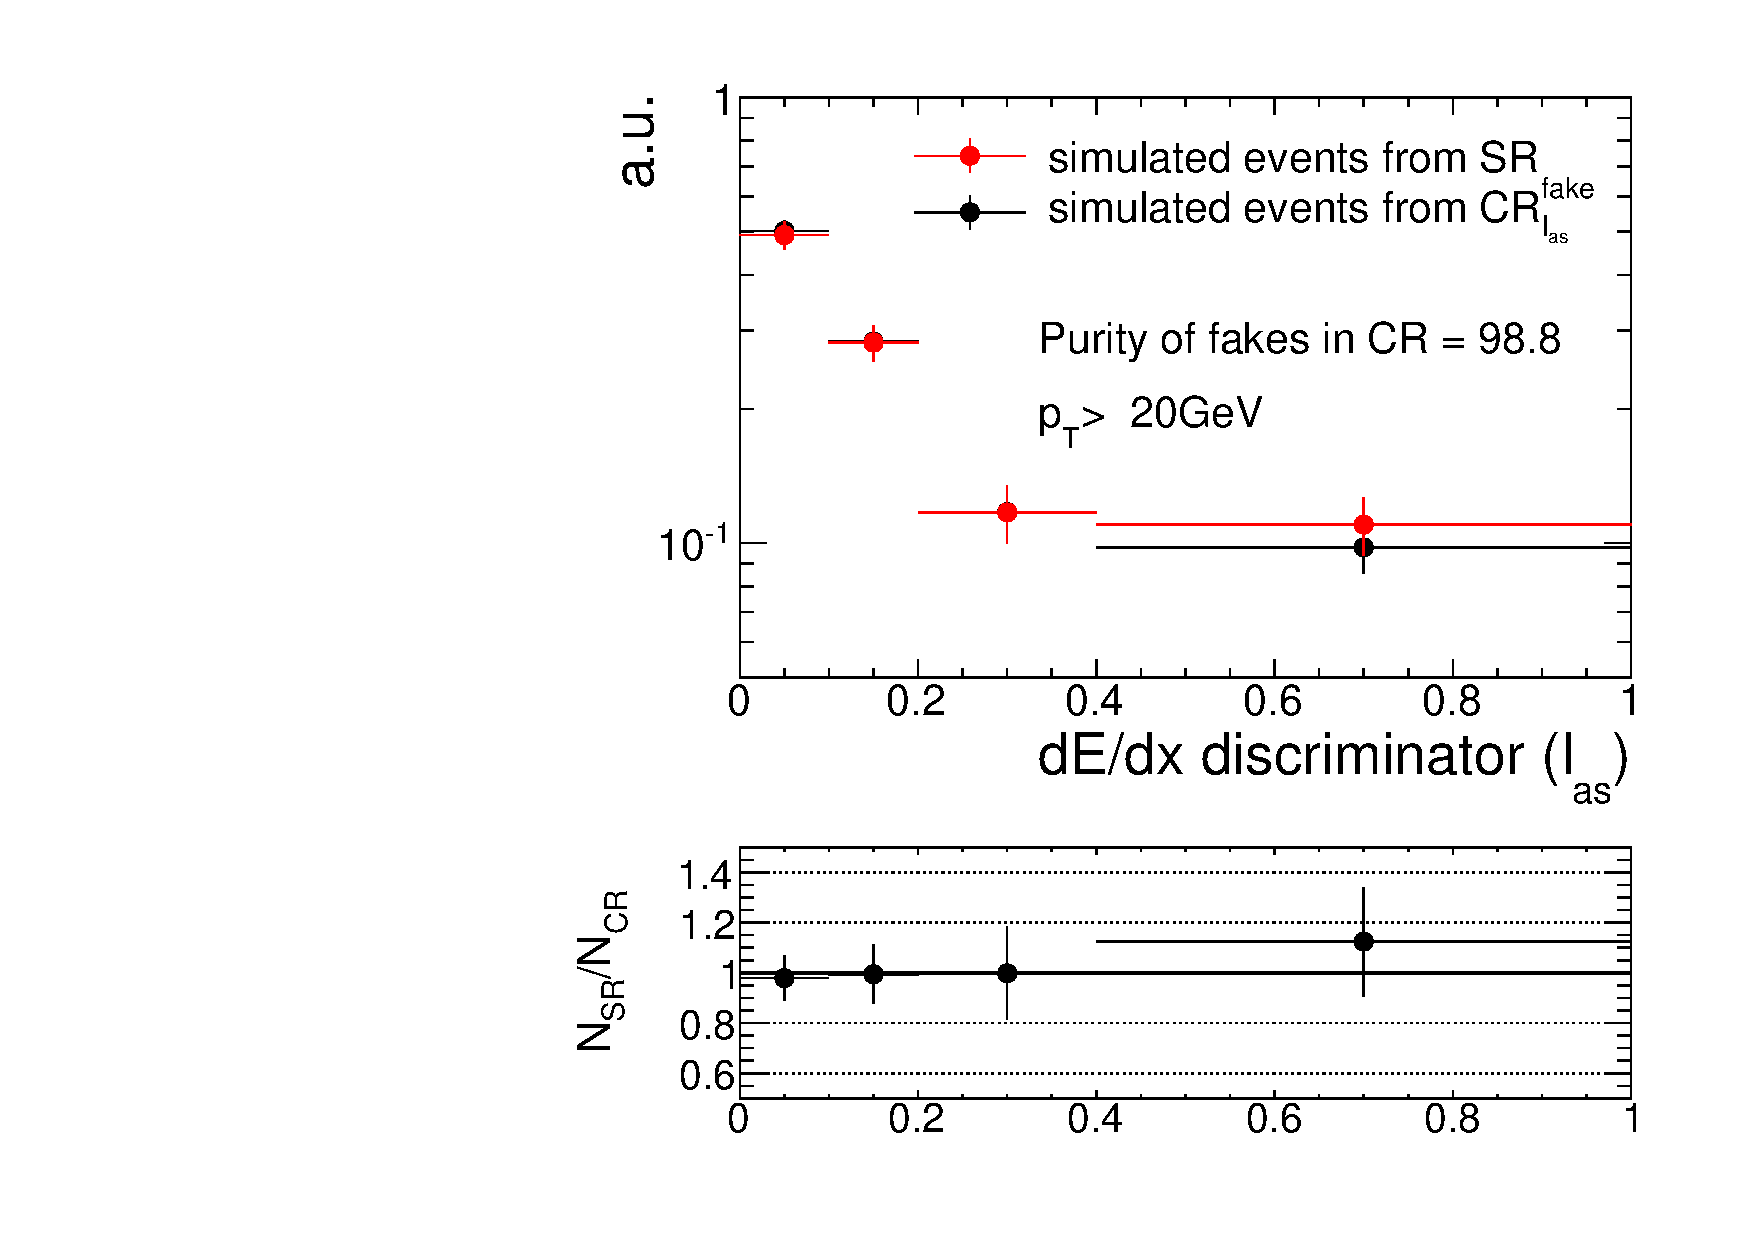
\includegraphics[width=0.49\textwidth]{figures/analysis/Background/hASmi_SRbinning_d0Inverted_fakes_ECalaoLe5_trackPtGt20_MC_CR_MC_SR.pdf}
    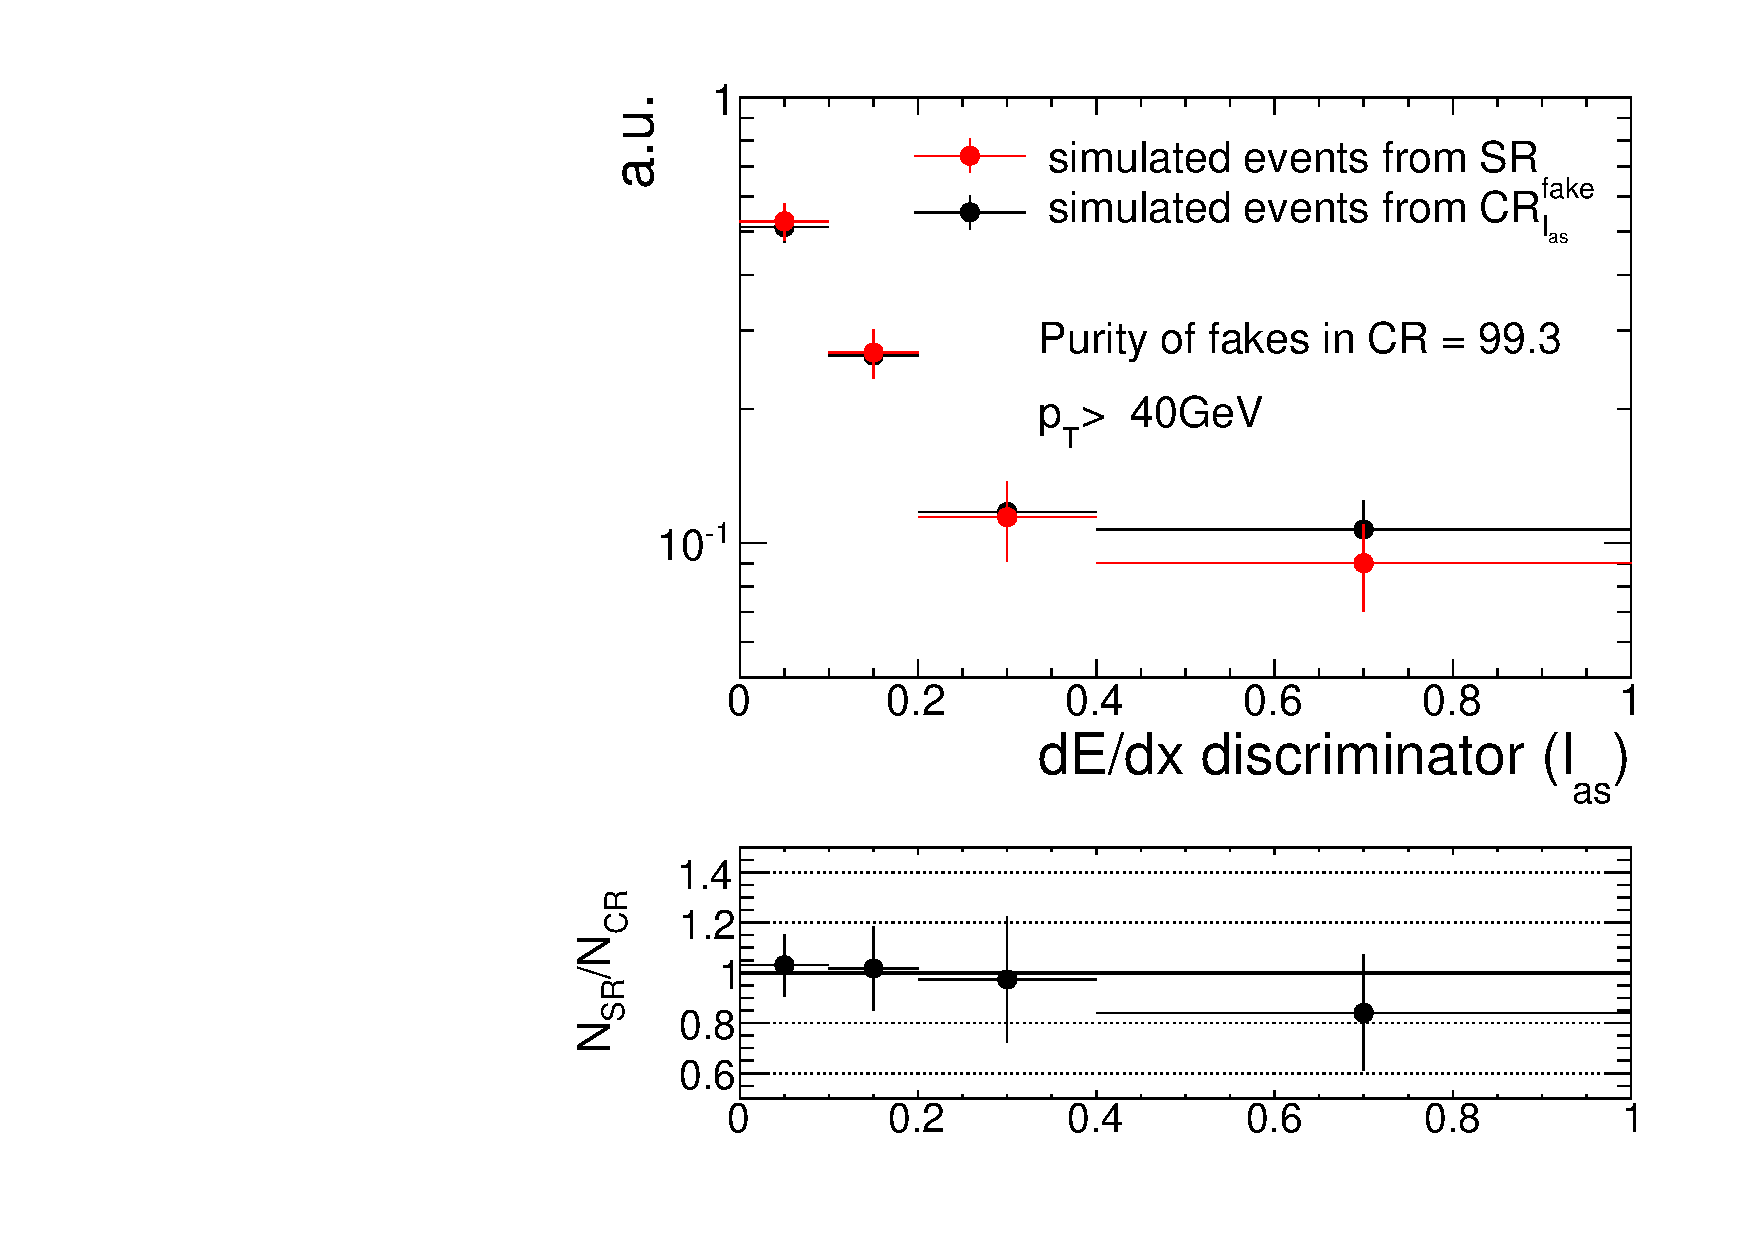
\includegraphics[width=0.49\textwidth]{figures/analysis/Background/hASmi_SRbinning_d0Inverted_fakes_ECalaoLe5_trackPtGt40_MC_CR_MC_SR.pdf}
  \end{tabular}
  \caption{Comparison of the \ias shape between CR$_{\ias}^{\text{fake}}$ and the signal region for two different track \pt cuts of 20\gev (left) and 40\gev (right). To enhance the statistical precision only the track selection is applied.}
  \label{fig:IasSRCRFakes}
\end{figure}

The \ias shape is almost identical in the signal and in the control region which makes the definition of the control region perfectly suited for the purpose to estimate the \ias shape from CR$_{\ias}^{\text{fake}}$ in data.
The differences between the both region will be taken as systematic uncertainty into account (discussed in Section~\ref{sec:FakeIasUncertainty}).
%%%%%%%%%%%%%%%%%%%%%%%%%%%%%%%%%%%%%%%%%%%%%%%%%%%%%%%%%%%%%%%%%%%%%%%%%%%%%%%%%%%%%%%%%%%%%%%%%%%%%%%%%%%%%%%%%%%%%%%%%%%%%%%%%%%%%%%%%%%%%%%%%%%%%%%%%%%%%%%%%%%%%%%%%%%%%%%%%%%%
%%%%%%%%%%%%%%%%%%%%%%%%%%%%%%%%%%%%%%%%%%%%%%%%%%%%%%%%%%%%%%%%%%%%%%%%%%%%%%%%%%%%%%%%%%%%%%%%%%%%%%%%%%%%%%%%%%%%%%%%%%%%%%%%%%%%%%%%%%%%%%%%%%%%%%%%%%%%%%%%%%%%%%%%%%%%%%%%%%%%
%%%%%%%%%%%%%%%%%%%%%%%%%%%%%%%%%%%%%%%%%%%%%%%%%%%%%%%%%%%%%%%%%%%%%%%%%%%%%%%%%%%%%%%%%%%%%%%%%%%%%%%%%%%%%%%%%%%%%%%%%%%%%%%%%%%%%%%%%%%%%%%%%%%%%%%%%%%%%%%%%%%%%%%%%%%%%%%%%%%%

\section{Leptonic background}
\label{sec:LeptonicBkg}

The leptonic background of the here presented search is caused by non-reconstructed leptons which undergo hence the lepton veto selection.
However, at least non-reconstructed electrons or taus should in principle deposit enough energy in the calorimeters such that they can still be vetoed by the calorimeter isolation requirement.
As muons don't deposit much energy in the calorimeters, this reason does not hold for them.
In the following, the sources of the three different leptonic backgrounds shall be characterised.

\subsection*{Electrons}
To avoid the background source from unreconstructed electrons, all tracks pointing to a dead or noisy ECAL cell, to an ECAL intermodule gap, or to the region between ECAL barrel and encap at $1.42<|\eta|<1.65$ are vetoed, 
as described in Section~\ref{sec:AnalysisSelection}.
By this selection, almost all electrons are efficiently rejected.
In the simulated \WJets sample only one simulated event remains that pass all candidate track selection criteria and for which the candidate track can be matched to a generator-level electron.
This event is visualised in Fig~\ref{fig:LostElectron}. 
\begin{figure}[!t]
  \centering 
  \begin{tabular}{c}
    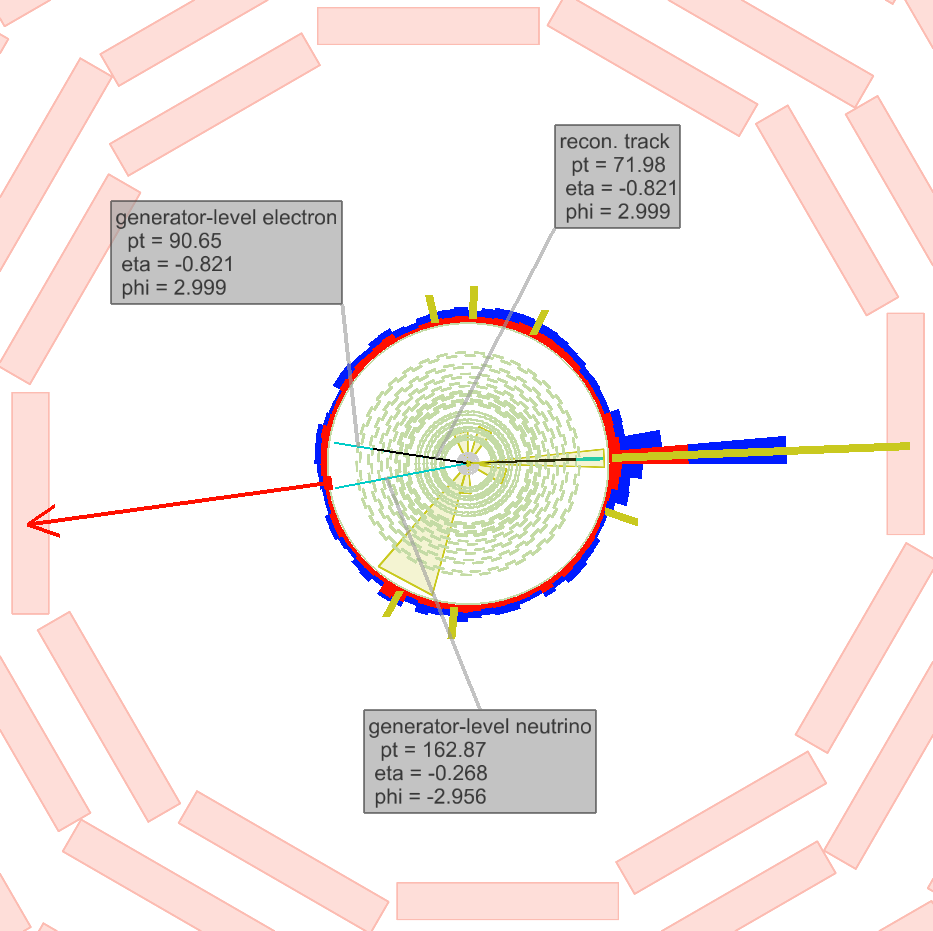
\includegraphics[width=0.49\textwidth]{figures/analysis/Electron_lumi_279317_event_111637553.png}
  \end{tabular}
 \caption{Visualisation of an $W\rightarrow e\nu_e$ event contributing to the SM background. 
           In light blue the generator-level particles $e$ and $\nu_e$ of the $W$ decay are shown. 
           The $\nu_e$, only weakly interacting does not show any signature in the detector, whereas the electron ($\pt\simeq 90\gev$) leaves a track (black line) with \mbox{$\pt\simeq 70\gev$} in the tracker. 
           No ECAL energy deposits in the direction of the electron are visible. 
           This is caused by the fact that the corresponding ECAL energy deposits were not read out in this event.
           An ISR jet ($\pt\simeq 230\gev$) causes the \met (read arrow) in the event. }
  \label{fig:LostElectron}
\end{figure}
 
In this event no energy deposits in the ECAL are read out, which suggests, that this ECAL tower was neither working properly in 2012.
Additionally, electrons can do bremsstrahlung which can change the direction of the electron significantly.
Thus, the energy deposits in the ECAL can possibly not be matched to the original electron.

\subsection*{Taus}
Taus are contributing to the leptonic background through the hadronic decay of a tau lepton to one charged pion $\tau\rightarrow\pi^{\pm}\nu$.
Other decay modes of the tau lepton are suppressed by the track isolation criterion.
Unreconstructed taus typically don't deposit energy in the HCAL or ECAL, thus fail reconstruction.
They can therefore also easily bypass the calorimeter isolation criterion.
Because of nuclear interactions in the tracker, pions often result in short reconstructed tracks that can easily be highly mismeasured in \pt.
Thus, taus can also contribute even when imposing a tighter selection in the transverse momentum.
Such an event is shown in Fig.~\ref{fig:LostTau}.  
\begin{figure}[!tb]
  \centering 
  \begin{tabular}{c}
    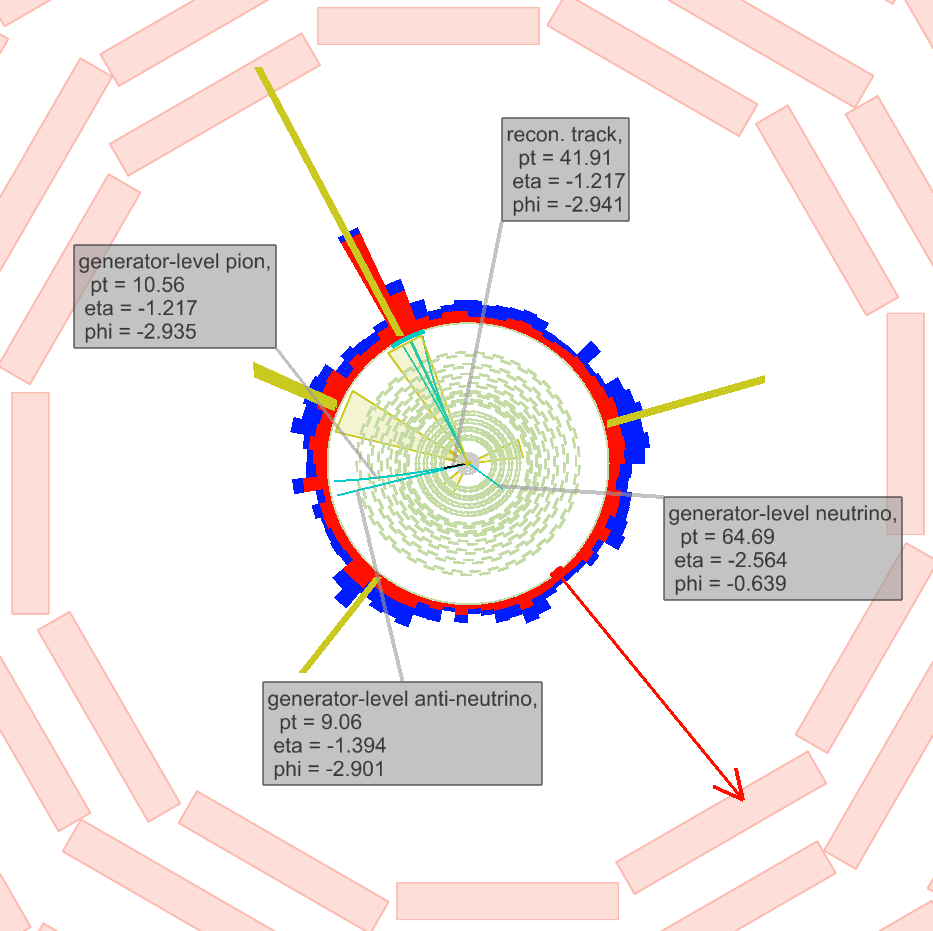
\includegraphics[width=0.49\textwidth]{figures/analysis/Background/LostTau_lumi_20940_event_8369426.png}
  \end{tabular}
  \caption{Visualisation of a $W^{+}\rightarrow \tau^{+}\nu_{\tau} \rightarrow \pi^{+}\bar{\nu}_{\tau} \nu_{\tau} $ event contributing to the SM background. 
           In light blue the generator-level particles $\pi^{+}$, $\bar{\nu}_{\tau}$ and $\nu_{\tau}$ are shown.
           The transverse momentum of the generator-level pion is only $\pt\sim10\gev$, but because the reconstructed track (black line) is very short, it leads to a high mismeasurement of the track \pt of $\sim40\gev$.
           The shortness of the track is caused by nuclear interactions of the pion.
           As no corresponding ECAL or HCAL energy deposits are measured the reconstruction of the pion fails.}
  \label{fig:LostTau}
\end{figure}

\subsection*{Muons}
Muons can fail reconstruction when they are pointing towards a bad cathode strip chamber.
This is taken into account in the candidate track selection.
However, some of the muons still fail reconstruction when they fall within the gap between stations 0 and 1 of the DT system at $|\eta|=0.25$.
The muon reconstruction efficiency drops from around 99\% to a value of around 94\% as shown in~\cite{bib:CMS:DT_Thesis,bib:CMS:DT_8TeV_AN}.
This possibility is illustrated in a simulated event shown in Fig~\ref{fig:LostMuon}.


In~\cite{bib:CMS:DT_Thesis,bib:CMS:DT_8TeV_AN} events are rejected when the track is pointing in a region of $0.15<|\eta|<0.35$.
In this search, this cut was omitted to maximise signal acceptance. 
Due to the additional selection in \ias, muons can easily be efficiently suppressed.
E.g. in the event example shown in Fig~\ref{fig:LostMuon}, the muon has an \ias value of about 0.007.\\


In general, all leptons are minimal ionising.
However, as electrons are much lighter compared to muons or pions, they loose more energy also via radiative effects.
Still, all three lepton types loose much less energy compared to hypothetical new heavy particles.
To have the possibility to make an optimisation in the two main discriminating variables \pt and \ias, the background estimation methods are designed to work for all different \pt and \ias selection cuts.
%A comparison of the \ias distribution for all four different background sources is shown in Fig~\ref{fig:IasDist}.
\begin{figure}[!tb]
  \centering 
  \begin{tabular}{c}
    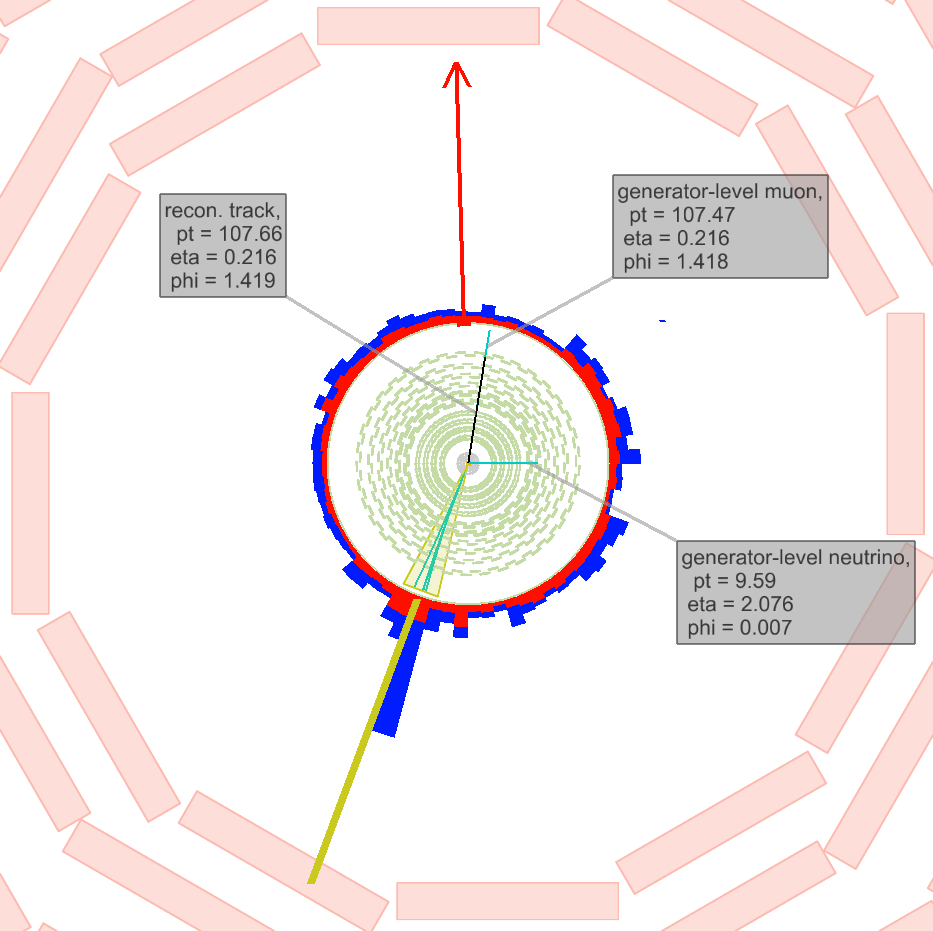
\includegraphics[width=0.49\textwidth]{figures/analysis/Background/LostMuon_Lumi_456307_event_182377157.png}
  \end{tabular}
  \caption{Visualisation of an $W\rightarrow \mu\nu_{\mu}$ event contributing to the SM background. 
           In light blue the generator-level particles $\mu$ and $\nu_{\mu}$ of the $W$ decay are shown. 
           The muon is pointing to the $\eta$-region between stations 0 and 1 of the DT system at $|\eta|\sim0.25$.
           In this region the muon reconstruction is less effcient. No signal in the muon chambers are visible. Therefore the  muon could not be reconstructed.}
  \label{fig:LostMuon}
\end{figure}

%\begin{figure}[!tb]
%  \centering 
%  \begin{tabular}{c}
%    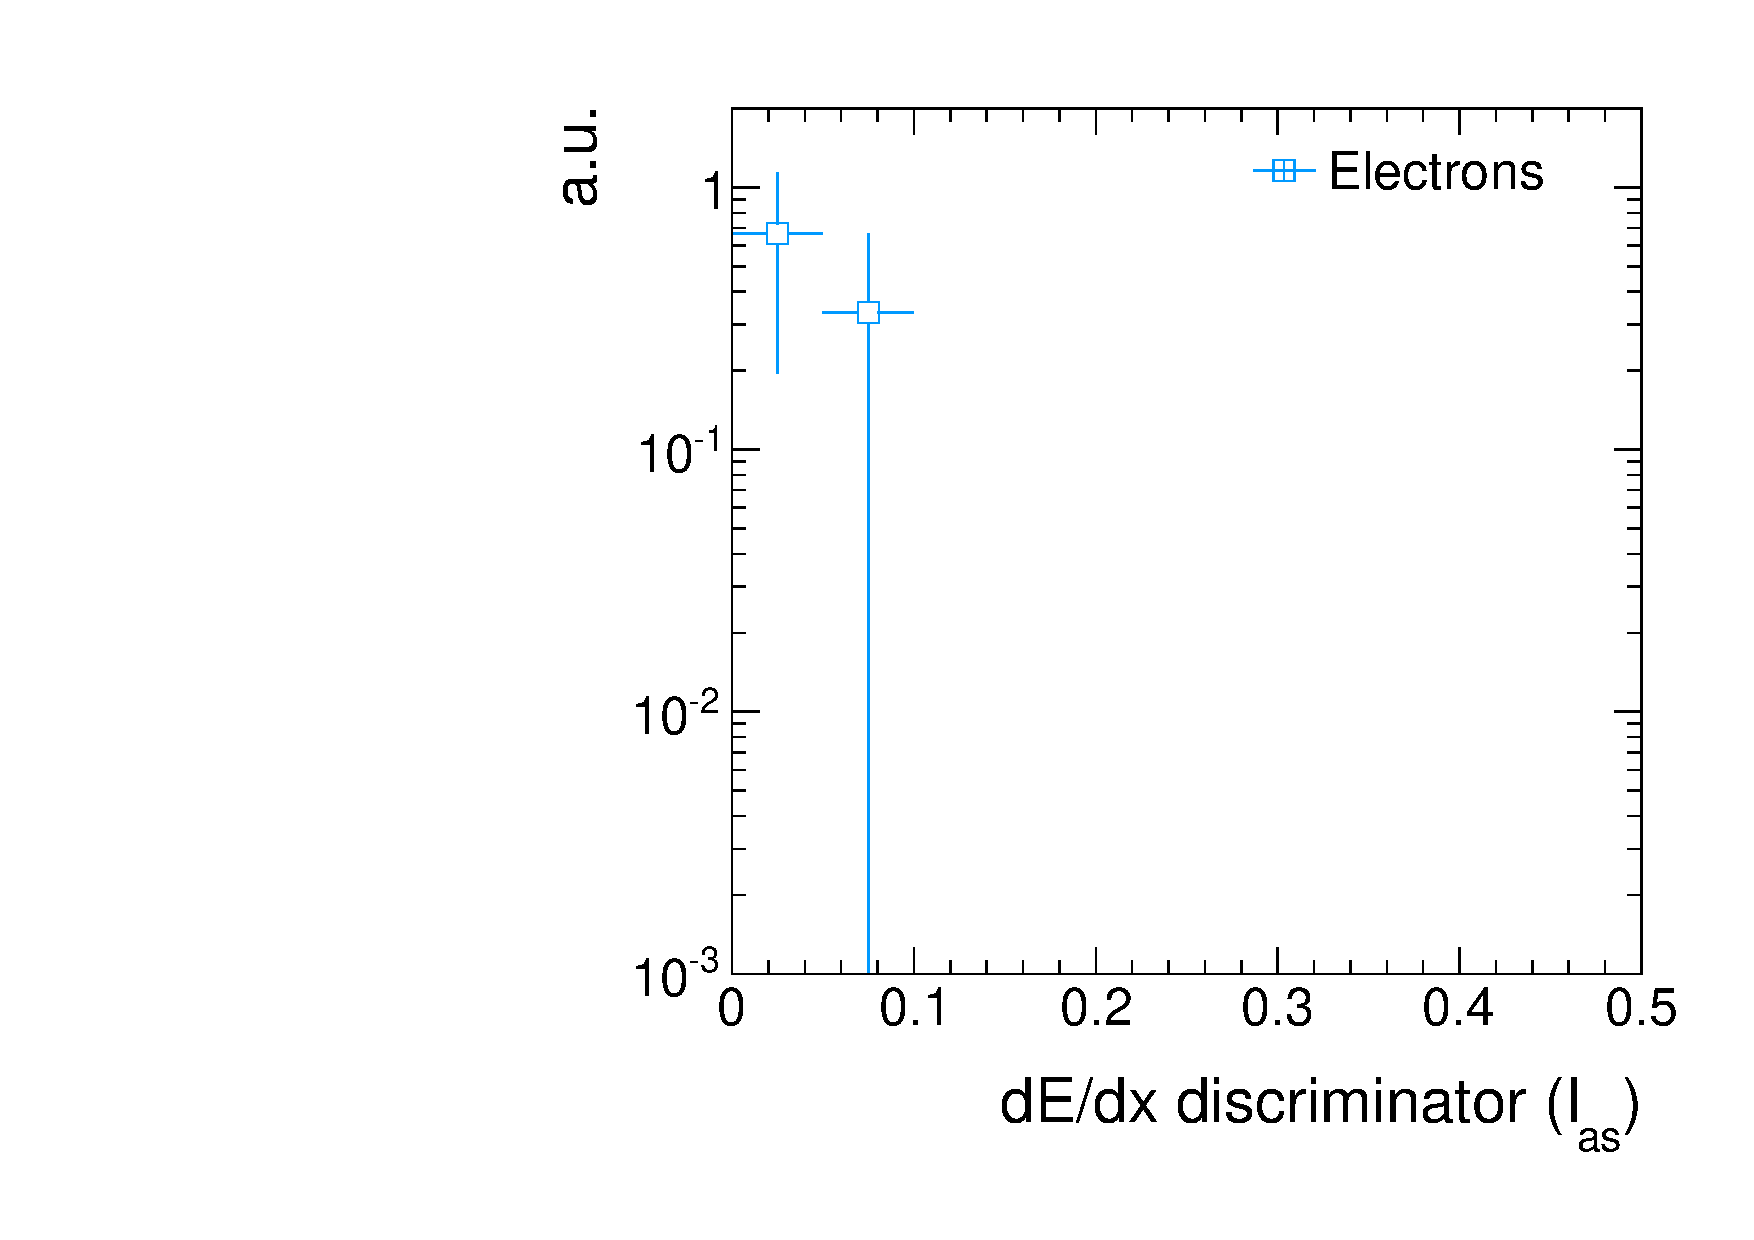
\includegraphics[width=0.33\textwidth]{figures/analysis/Background/IasDistributionForElecs.pdf}
%    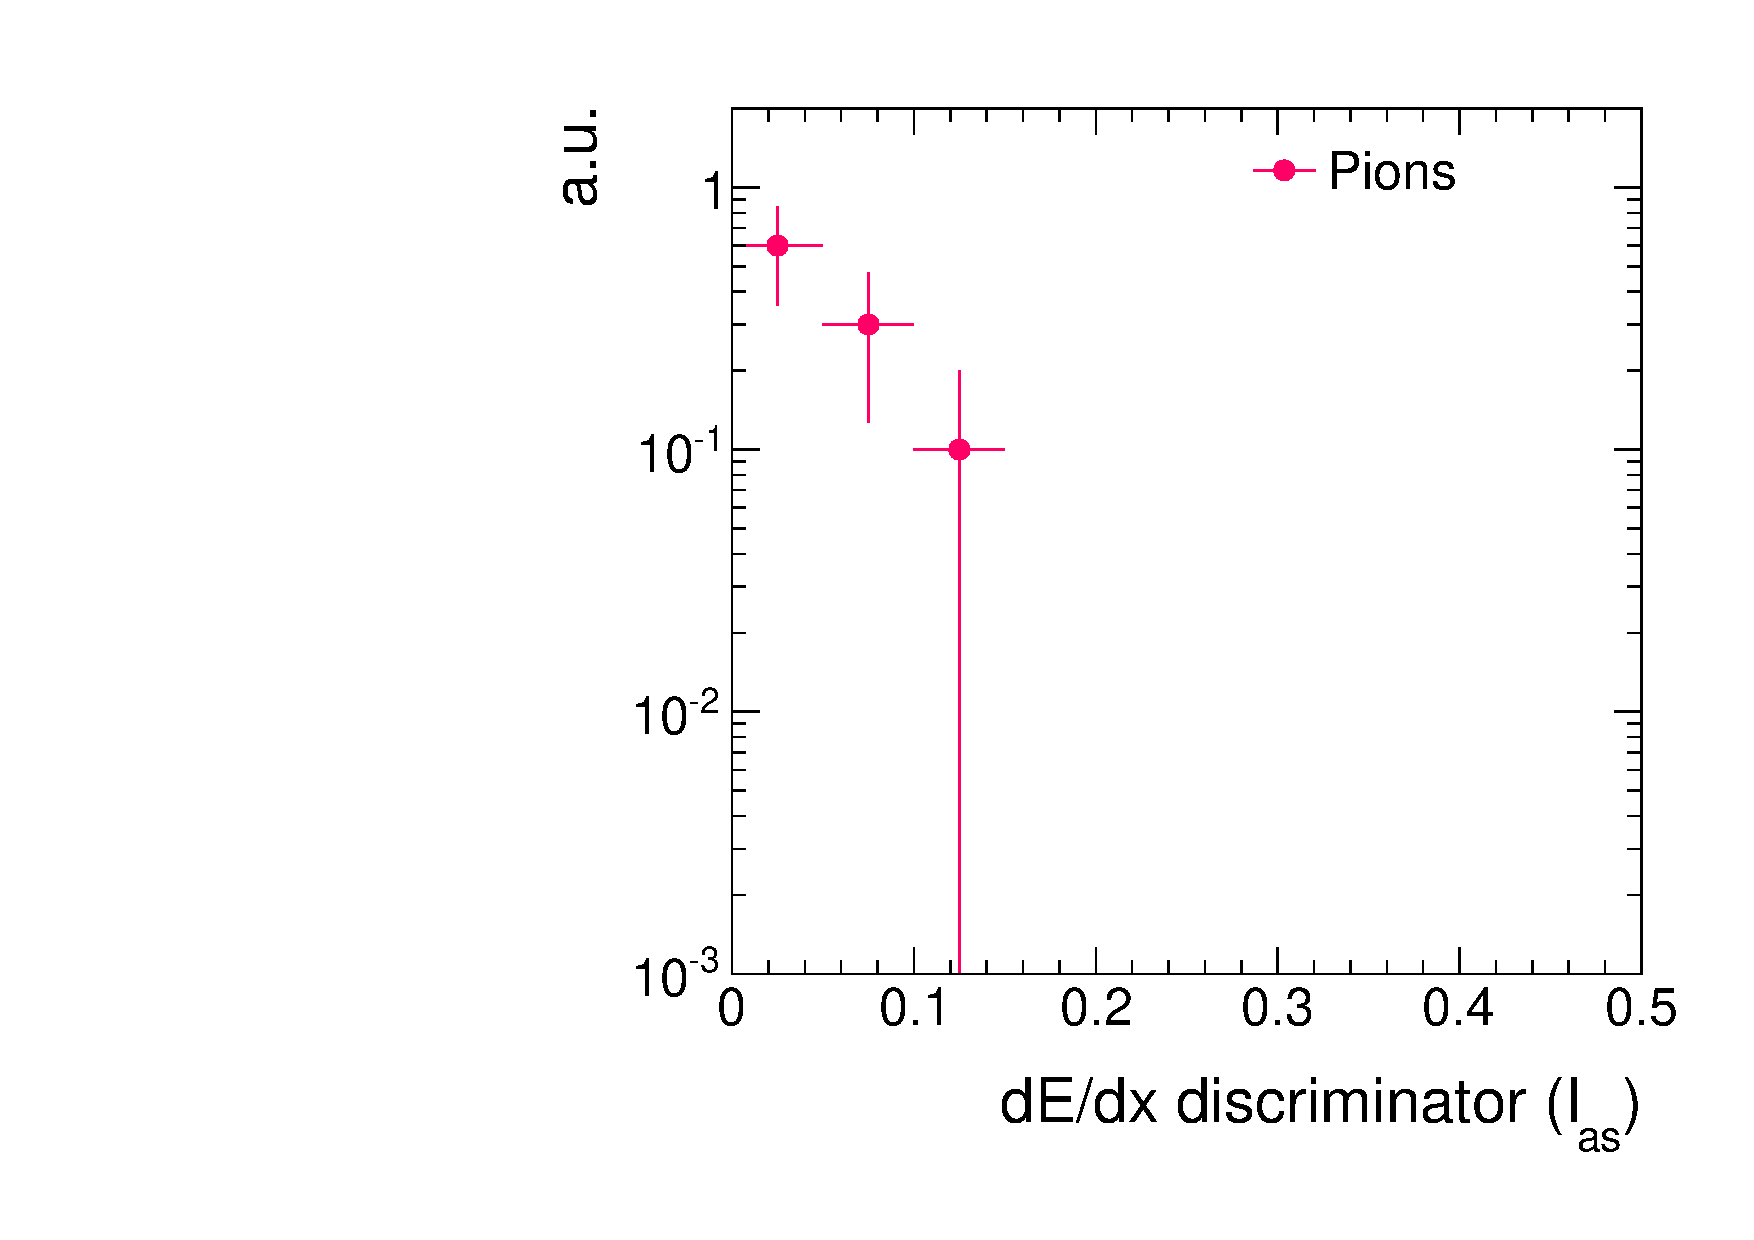
\includegraphics[width=0.33\textwidth]{figures/analysis/Background/IasDistributionForPions.pdf}
%    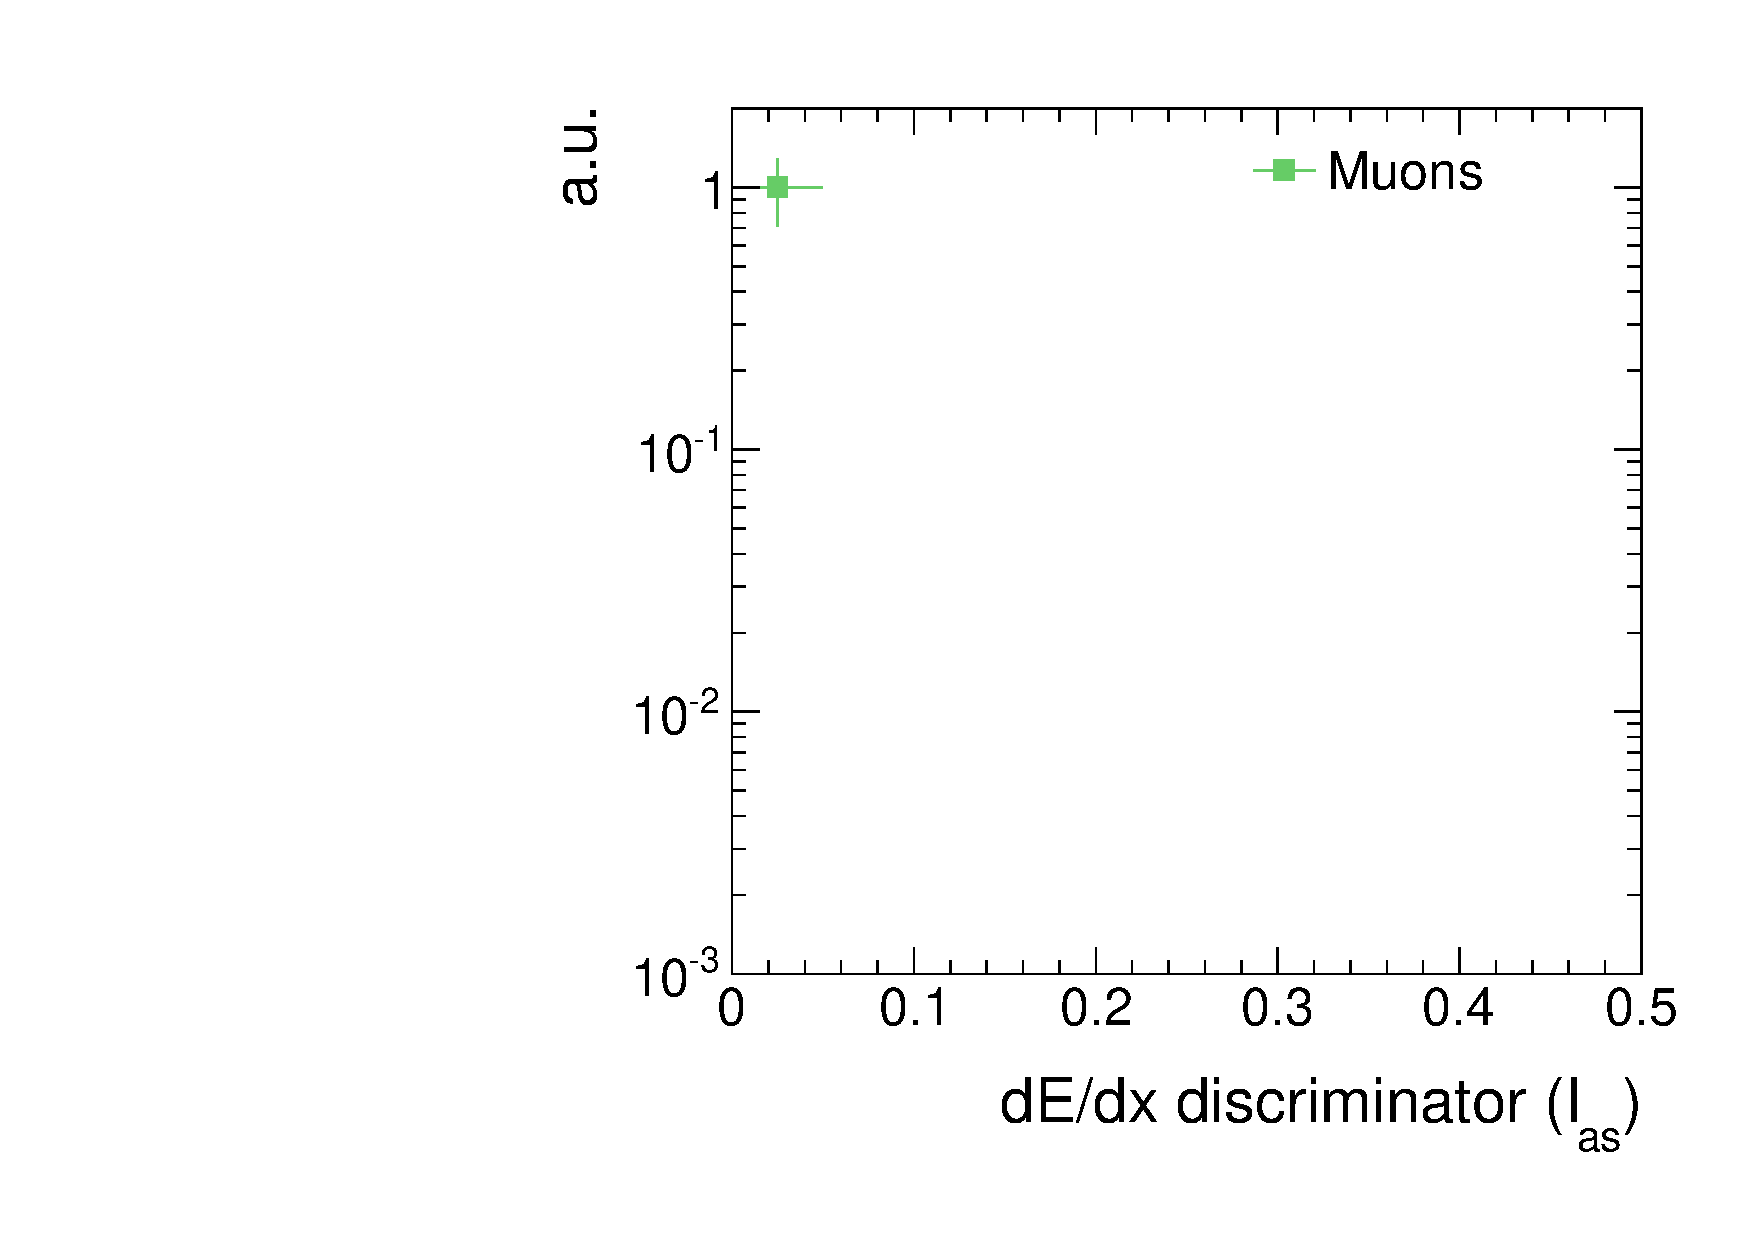
\includegraphics[width=0.33\textwidth]{figures/analysis/Background/IasDistributionForMuons.pdf}
%  \end{tabular}
%  \caption{Normalised \ias distribution for electrons (left), pions (middle) and muons (right). 
%           For all leptons the \ias distribution is rapidly falling.}
%  \label{fig:IasDist}
%\end{figure}


Also for the leptonic background the estimation method is splitted into two parts.
First, the estimation of the inclusive background without \ias information.
Second, the estimation of the \ias shape for all three leptonic background sources.


\subsection*{Inclusive leptonic background estimation}
The inclusive (without \ias information) lepton background estimation method follows closely the background estimation method used in~\cite{bib:CMS:DT_Thesis,bib:CMS:DT_8TeV_AN}.

In order to estimate the number of events in the signal region originating from unreconstructed leptons, information from simulated events is used.
With the help of simulated \WJets events, the ratio between the number of events in the signal region with the selected track matched to a generator-level lepton $N_{SR}^{\text{trk matched to lepton}_i}$
 and the number of events in the control region $N_{CR}^{\text{lepton}_i\text{ veto inverted}}$ with the lepton veto inverted is determined.
For muons, this lead to the following expression
\begin{equation*}
\rho_{\text{MC}}^{\mu} = \frac{N_{\text{SR,MC}}^{\text{trk matched to }\mu}}{N_{\text{CR,MC}}^{\mu \text{ veto inverted}}}.
\end{equation*}
Since for electrons and taus the reconstruction efficiency is highly correlated with the \ecalo selection requirement, the \ecalo requirement is additionnaly removed in the control regions for these two lepton types 
\begin{equation*}
\rho_{\text{MC}}^{e,\tau} = \frac{N_{\text{SR,MC}}^{\text{trk matched to }e,\tau}}{N_{\text{CR,MC}}^{e,\tau\text{ veto inverted}, \cancel{\ecalo<5\gev}}}.
\end{equation*}

In order to estimate the inclusive background for all three lepton types, the scaling factor $\rho_{\text{MC}}^{\text{lep}_i}$ is applied to the number of events in the lepton veto inverted control region measured in data.
Also in data the control region for electrons and taus is defined with the \ecalo requirement removed. 
Thus the inclusive number of background events is 
\begin{equation*}
N^{\mu \text{, inclusive in I$_{\text{as}}$}}_{\text{bkg}} = \rho_{\text{MC}}^{\mu} \cdot N_{\text{CR,data}}^{\mu\text{ veto inverted}}.
\end{equation*}
for muons, and 
\begin{equation*}
N^{e,\tau\text{, inclusive in I$_{\text{as}}$}}_{\text{bkg}} = \rho_{\text{MC}}^{e,\tau} \cdot N_{\text{CR,data}}^{e,\tau\text{ veto inverted}, \cancel{\ecalo<5\gev}}.
\end{equation*}
for electrons and taus.

This method relies on the simulation of the lepton reconstruction inefficiencies.
A possible wrong simulation is taken into account via a comparison of the lepton reconstruction efficiencies in data and simulation in \Zlep events which will be later explained in Section~\ref{sec:LeptonScaleUncertainty}.

To reduce the statistical uncertainty, the scale factor is calculated without applying the QCD suppression cuts. 
After the candidate track selection described in Section~\ref{sec:AnalysisSelection} (without QCD selection cuts), only one event remains in the simulated \WJets sample where the candidate track can be matched to an electron.
There are five track candidates that can be matched to a muon, and zero selected tracks that can be mactched to a pion.
The 68\% upper and lower limits on the inclusive background are estimated with the Neyman procedure~\cite{bib:PDG_2014}.
Table~\ref{tab:LeptonicResults} gives the result for the prediction of the inclusive leptonic background estimation for the candidate track selection from Section~\ref{sec:AnalysisSelection}.

\renewcommand{\arraystretch}{1.4}
\begin{table}[!h]
\centering
\caption{Scaling factor $\rho_{\text{MC}}$, number of events in the control region in data N$_{\text{CR,data}}$ and the resulting inclusive estimation N$_{\text{predicted}}$ after the candidate track selection.}
\label{tab:LeptonicResults}
\makebox[0.99\textwidth]{
\begin{tabular}{l|c |c| c }
\multicolumn{4}{c}{} \\
\toprule
                                                               &      scaling factor $\rho_{\text{MC}}$    &   N$_{\text{CR,data}}$         &  N$_{\text{predicted}}$   \\
\midrule
electrons                                                      &       $1.25^{+1.70}_{-0.77} 10^{-4}  $      & 60067                     & $7.49^{+10.19}_{-4.63}$     \\
muons                                                          &       $2.17^{+1.65}_{-0.93} 10^{-4}$        & 76664                     & $16.64^{+12.64}_{-7.12}$    \\
taus                                                           &       $< 2.13 10^{-2}$                  & 445                      &  $<9.46$ \\
\bottomrule
\end{tabular}}
\end{table}



\subsection*{\ias shape of leptonic background}
In order to get information about the \ias shape of electrons, muons and taus in the signal region, one need to find a control region where the shape is similar to that in the signal region.
The most natural control region, being the lepton veto inverted control region, cannot be used because the variable \ias is highly correlated to the lepton recontruction efficiency, as can be seen in Fig.~\ref{FIXME}.
Various other control regions were tested.
Unfortunately, the energy deposition is not only correlated to the reconstruction probability of the leptons but also to \ecalo, \pt and various other observables that were tested.
As no suitable control region exists where the \ias shape of the leptons is at least similar to the shape in the signal region, it is therefore decided to use the \ias information from simulation.
This introduces of course a large systematic uncertainty.
However, the corresponding systematic uncertainty is still smaller than taking the \ias shape from a control region in data.

In order to take into account the bias when taking \ias from simulation, a systematic uncertainty is estimated that address simulation-data differences of the \ias distributions.
This systematic uncertainty is discussed in Section~\ref{sec:LeptonIasUncertainty}.
%%%%%%%%%%%%%%%%%%%%%%%%%%%%%%%%%%%%%%%%%%%%%%%%%%%%%%%%%%%%%%%%%%%%%%%%%%%%%%%%%%%%%%%%%%%%%%%%%%%%%%%%%%%%%%%%%%%%%%%%%%%%%%%%%%%%%%%%%%%%%%%%%%%%%%%%%%%%%%%%%%%%%%%
%%%%%%%%%%%%%%%%%%%%%%%%%%%%%%%%%%%%%%%%%%%%%%%%%%%%%%%%%%%%%%%%%%%%%%%%%%%%%%%%%%%%%%%%%%%%%%%%%%%%%%%%%%%%%%%%%%%%%%%%%%%%%%%%%%%%%%%%%%%%%%%%%%%%%%%%%%%%%%%%%%%%%%%
\section{Background estimation validation}
\label{sec:BkgValidation}

The background estimation methods are exhaustively validated with the help of signal depleted control regions.
Various control regions were used for the validation.

First, to validate the estimation method of the leptonic background, a leptonic control region is defined by selecting only tracks with $\nhits>6$.
This reduces the fake contribution to a minimum.
Additionally in order to minimise signal contamination, the \ecalo requirement is inverted to $\ecalo>10\gev$.
The validation test for the candidate track selection with $\ecalo>10\gev$ and $\nhits>6$ is shown in Table~\ref{tab:LeptonicClosure}.
\renewcommand{\arraystretch}{1.4}
\begin{table}[!h]
\centering
\caption{Validation test of leptonic background estimation. Left: $\ecalo>10\gev$ and $\nhits>6$ (only statistical uncertainties are included). Right: $\ecalo>10\gev$, $\nhits>6$ and $\ias>0.2$}
\label{tab:LeptonicClosure}
\makebox[0.99\textwidth]{
\begin{tabular}{l|c |c}
\multicolumn{3}{c}{} \\
\toprule
                                                               &      Predicted Yield                       &   Data Yield          \\
\midrule
electrons                                                      &       $14.67^{+ 11.16}_{-6.29}$            &                \\
muons                                                          &       $7.99^{ + 10.90}_{-5.00}$            &            \\
taus                                                           &       $109.04^{+21.18}_{-16.58}$           &          \\
\midrule
Total bkg                                                      &       $132.68^{ + 26.31}_{-18.43}$         &  156        \\
\bottomrule
\end{tabular}
\hspace{10pt}
\begin{tabular}{l|c |c}
\multicolumn{3}{c}{} \\
\toprule
                                                               &      Predicted Yield                   &   Data Yield          \\
\midrule
electrons                                                      &       $0.0^{+ 0.07}_{-0.0}$               &                \\
muons                                                          &       $0.0^{+ 0.32}_{-0.0}$               &            \\
taus                                                           &       $0.0^{+ 0.38}_{-0.0}$               &          \\
\midrule
Total bkg                                                      &       $0.0^{+ 0.50}_{-0.0}$               &  1        \\
\bottomrule
\end{tabular}}
\end{table}\\


In order to validate the fake background, the \nhits selection cut is again removed.
As the inclusive fake background can only be estimated within the low calorimeter isolation region $\ecalo<5\gev$ or $\ecalo<10\gev$, 
the information about the number of fake tracks in the high \ecalo region is taken from the fake enriched control region.
In this control region, the ratio of $N_{\ecalo>10\gev}/N_{\ecalo<10\gev}$ is estimated and taken as a multiplicator to the number of events predicted from the $\ecalo<10\gev$ region.
In Table~\ref{tab:FakeClosure}, two different validation tests are shown, once an inclusive validation in \ias and once with an \ias selection of 0.2.
\renewcommand{\arraystretch}{1.4}
\begin{table}[!h]
\centering
\caption{Validation test of fake and leptonic background estimation methods (only statistical uncertainties are included). Left: $\ecalo>10\gev$ . Right: $\ecalo>10\gev$ and $\ias>0.2$}
\label{tab:FakeClosure}
\makebox[0.99\textwidth]{
\begin{tabular}{l|c |c}
\multicolumn{3}{c}{} \\
\toprule
                                                               &      Predicted Yield                   &   Data Yield          \\
\midrule
Electrons                                                      &     $59.92^{ + 16.11}_{ - 11.85}$                 &                \\
Muons                                                          &     $8.04^{ + 10.97}_{ - 5.03}$                &            \\
Taus                                                           &     $173.06^{+ 24.62}_{- 20.23}$               &          \\
Fakes                                                          &     $67.98^{+ 11.57}_{- 11.57}$               &          \\
\midrule
Total bkg                                                      &     $309.00^{+ 33.46} _{- 26.62}$             &  324        \\
\bottomrule
\end{tabular}
\hspace{10pt}
\begin{tabular}{l|c |c}
\multicolumn{3}{c}{} \\
\toprule
                                                               &      Predicted Yield                       &   Data Yield          \\
\midrule
Electrons                                                      &       $0.75^{ + 0.36}_{ - 0.25}$            &                \\
Muons                                                          &       $0.00^{ + 0.32}_{- 0.00}$            &            \\
Taus                                                           &       $2.33^{ + 0.74}_{- 0.55}$            &          \\
Fakes                                                          &       $11.72^{ + 2.79}_{- 2.79}$            &          \\
\midrule
Total bkg                                                      &       $14.80^{ + 2.92}_{- 2.85}$            &  16        \\
\bottomrule
\end{tabular}}
\end{table}\\




The validation is done for different selections in \pt and \ias.
All validation tests show good agreement.

Still, systematic uncertainties need to be estimated.
The sources of systematic uncertainties and how they are estimated will be explained in the following section.


\section{Systematic uncertainties}
\label{sec:SysUncertaintiesBkg}

The corresponding systematic uncertainties for the background estimation methods, are the uncertainty on the fake rate $\rho_{\text{fake}}$, the uncertainty of shape differences in the \ias distribution between the signal region and the fake control region CR$_{\ias}^{\text{fake}}$, the uncertainty on the leptonic scale factor $\rho_{\text{MC}}^{\text{lep}_i}$ determined with simulated events, and the uncertainty of the shape differences between simulation and real data of the leptonic background.  
\subsection{Uncertainty on the fake rate}
\label{sec:FakeRateUncertainty}
The uncertainty on the fake rate $\rho_{\text{fake}}$ is determined with a comparison of the fake rate in \WJets and \Zlep events in simulation.
\subsection{Uncertainty on the fake track \ias shape}
\label{sec:FakeIasUncertainty}
\subsection{Uncertainty on the leptonic scale factor}
\label{sec:LeptonScaleUncertainty}
\subsection{Uncertainty on the leptonic \ias shape}
\label{sec:LeptonIasUncertainty}

%%%%%%%%%%%%%%%%%%%%%%%%%%%%%%%%%%%%%%%%%%%%%%%%%%%%%%%%%%%%%%%%%%%%%%%%%%%%%%%%%%%%%%%%%%%%%%%%%%%%%%%%%%%%%%%%%%%%%%%%%%%%%%%%%%%%%%%%%%%%%%%%%%%%%%%%%%%%%%%%%%%%%%%
%%%%%%%%%%%%%%%%%%%%%%%%%%%%%%%%%%%%%%%%%%%%%%%%%%%%%%%%%%%%%%%%%%%%%%%%%%%%%%%%%%%%%%%%%%%%%%%%%%%%%%%%%%%%%%%%%%%%%%%%%%%%%%%%%%%%%%%%%%%%%%%%%%%%%%%%%%%%%%%%%%%%%%%
